% ===================== AUTHOR TO-DO BEFORE SUBMISSION =====================
% 1. Fill the placeholders marked [to be completed] (affiliation, e-mail, CRediT, funding, AI-use statement).
% 2. Set \journal{...} to the target journal.
% 3. Figures 3-7 and Fig. 1 still show "GT"/"gas turbine" labels: regenerate them with "GT"/"gas turbine".
% 4. Verify every reference against its source (see the reply notes); Table I entries for works not verified by the editor.
% 5. Re-run the HiGHS reference-tree values if you prefer one solver for all tables (Tables V-X use HiGHS).
% ===========================================================================
\documentclass[5p,times,twocolumn]{elsarticle}
\usepackage{amsmath,amssymb,amsfonts}
\usepackage{graphicx}
\usepackage[T1]{fontenc}
\usepackage{lmodern}
\usepackage{textcomp}
\usepackage{eurosym}
\usepackage{xcolor}
\usepackage{booktabs}
\usepackage{multirow}
\usepackage{makecell}
\usepackage{enumitem}
\usepackage{tabularx}
\usepackage{array}
\usepackage{url}
\usepackage{hyperref}
\usepackage{comment}
\usepackage{tabularx}
\usepackage{booktabs}
\usepackage{array}
\usepackage{xurl}



\usepackage{needspace}

% ---- Nomenclature environment ----
\newenvironment{nomlist}{%
  \begingroup\footnotesize
  \list{}{%
    \setlength{\labelwidth}{0.27\columnwidth}%
    \setlength{\labelsep}{4pt}%
    \setlength{\leftmargin}{\dimexpr\labelwidth+\labelsep\relax}%
    \setlength{\itemsep}{0.5pt}\setlength{\parsep}{0pt}%
    \setlength{\topsep}{1pt}\setlength{\partopsep}{0pt}%
    \renewcommand{\makelabel}[1]{##1\hfil}}%
}{\endlist\endgroup}

\newcommand{\nomheading}[1]{%
  \Needspace{4\baselineskip}%
  \par\vspace{3pt}\noindent{\footnotesize\bfseries\itshape #1}\par\vspace{1pt}}
\newcommand{\nomitem}[2]{\item[#1] #2}



\journal{Applied Energy}

\begin{document}

\begin{frontmatter}

\title{Multi-Market Participation of a Large Industrial Prosumer with Battery Storage and Gas Turbine: A Three-Stage Stochastic Co-Scheduling Approach}

\author[inst1]{Sreelatha Aihloor Subramanyam\corref{cor1}}
\author[inst1]{Amjad Anvari-Moghaddam}
\cortext[cor1]{Corresponding author. E-mail: sasu@energy.aau.dk}
\affiliation[inst1]{organization={Department of Energy, Aalborg University, Aalborg, Denmark}}

\begin{abstract}
Energy-intensive batch plants such as smelters and foundries combine large, partly shiftable furnace loads with on-site assets, typically thermal units such as a gas turbine and increasingly a battery, and can trade in several electricity markets. Yet scheduling studies rarely include multi-market participation, and bidding studies rarely include discrete production constraints. This paper proposes a three-stage stochastic MILP, with an optional CVaR risk term, and reports risk-neutral results. In Stage 1, before prices are known, it schedules the non-interruptible furnace batches, commits the gas turbine, and sets monotone Day-Ahead offer curves and an hourly spinning up-reserve capacity. Stages 2 and 3 then adjust the plant through Intraday trading, battery operation and imbalance settlement. A representative plant (5 furnaces, 30 tasks, 25~MW gas unit, 40~MW / 200~MWh battery) is demonstrated in real prices of DK1 Day-Ahead and spinning reserve capacity. On eight scenario trees built from the preceding 90 days, Intraday trading and up-reserve reduce expected net operating cost by 2.9--11.9\% (mean 7.1\%) against Day-Ahead only, and the reserve share follows the spinning reserve price, which fell during the year. With Stage-1 decisions fixed and evaluated on seven following days, the saving is 3.7\% (\euro 5,403). On the reference tree the battery lowers expected operating cost by \euro 10.5k per day (7.0\%), 83\% of it from Day-Ahead and Intraday arbitrage and 17\% from reserve; it supplies about 90\% of the reserve benefit, and the reserve saving stays at \euro 1.9--2.1k for round-trip efficiencies of 76--90\% and degradation costs of \euro 2.5--10/MWh. The stochastic plan beats the deterministic expected-value (EV) plan by 0.7--1.3\% (mean 0.9\%), above solver noise on 10 of 11 trees. Planning production separately from the market offers raises the cost by 0.4--1.4\% on three of the four earlier trees; on the fourth tree and on the reference tree the difference is within the solver tolerance.
\end{abstract}

\begin{highlights}
\item Three-stage stochastic MILP couples furnace batches, gas turbine and battery
\item Multi-market trading cuts expected operating cost by 2.9--11.9\% on real DK1 prices
\item Realized saving on seven actual days with the Stage-1 plan fixed is 3.7\%
\item Battery gives 83\% of its value from arbitrage; reserve share is robust to efficiency
\item Stochastic plan beats the deterministic expected-value plan by 0.7--1.3\% on 10 of 11 trees
\end{highlights}

\begin{keyword}
Battery energy storage \sep Industrial prosumer \sep Stochastic programming \sep Reserve market \sep Day-ahead and intraday markets \sep Batch production scheduling \sep Value of the stochastic solution \sep Gas turbine
\end{keyword}

\end{frontmatter}


\section*{Nomenclature}

\nomheading{Sets and indices}
\begin{nomlist}
\nomitem{$t\in T$}{Time periods over the 24-h horizon ($|T|=24$)}
\nomitem{$m\in M$}{Industrial machines/furnaces ($|M|=5$)}
\nomitem{$p\in P$}{Manufacturing tasks ($|P|=30$)}
\nomitem{$n\in N$}{Batch sequence slots ($|N|=10$)}
\nomitem{$s\in S$}{Price scenarios ($|S|=3$)}
\nomitem{$w\in W$}{Real-time imbalance and activation scenarios ($|W|=3$)}
\end{nomlist}

\nomheading{Parameters}
\begin{nomlist}
\nomitem{$td_{m,p}$}{Processing duration of task $p$ on machine $m$ (h)}
\nomitem{$d_{m,p}$}{Electrical power demand of task $p$ on machine $m$ (MW)}
\nomitem{$t_{\mathrm{buffer}}$}{Inter-batch setup, cleaning and cooling buffer (h)}
\nomitem{$Y_p$}{Finished-goods yield of task $p$ (units)}
\nomitem{$N_{\max}$}{Maximum warehouse capacity (units)}
\nomitem{$N_0$}{Initial inventory (units)}
\nomitem{$n_{\mathrm{prod,dem},t}$}{Product delivery commitment in hour $t$ (units/h)}
\nomitem{$P_{\mathrm{GT,min}}$}{Minimum gas turbine output (MW)}
\nomitem{$P_{\mathrm{GT,max}}$}{Maximum gas turbine output (MW)}
\nomitem{$C_0^{\mathrm{GT}}$}{Baseline gas turbine cost (\euro/MWh)}
\nomitem{$C_m^{\mathrm{GT}}$}{Cost of gas turbine output block $m$ (\euro/MWh)}
\nomitem{$P_{\max}^{\mathrm{BESS}}$}{Maximum BESS power (MW)}
\nomitem{$E_{\max}^{\mathrm{BESS}}$}{BESS energy capacity (MWh)}
\nomitem{$C_{\mathrm{TP}}$}{BESS throughput degradation cost (\euro/MWh)}
\nomitem{$\lambda_{\mathrm{buy},t}^{\mathrm{DA}}$}{Day-ahead purchase price (\euro/MWh)}
\nomitem{$\lambda_{\mathrm{sell},t}^{\mathrm{DA}}$}{Day-ahead sale price (\euro/MWh)}
\nomitem{$r^{+}$}{Imbalance price ratio for surplus energy ($r^{+}\le 1$)}
\nomitem{$r^{-}$}{Imbalance price ratio for deficit energy ($r^{-}\ge 1$)}
\end{nomlist}

\nomheading{Decision variables}
\begin{nomlist}
\nomitem{$ts_{m,n}$}{Start time of batch slot $n$ on machine $m$ (h)}
\nomitem{$X_{m,n,p}$}{Binary assignment of task $p$ to slot $n$ on machine $m$}
\nomitem{$u_{\mathrm{GT},t}$}{Gas turbine commitment status (binary)}
\nomitem{$x_{\mathrm{GT},t}$}{Gas turbine start-up indicator (binary)}
\nomitem{$y_{\mathrm{GT},t}$}{Gas turbine shut-down indicator (binary)}
\nomitem{$P_{\mathrm{buy},t}^{\mathrm{DA}}$}{Day-ahead electricity purchase (MW)}
\nomitem{$P_{\mathrm{sell},t}^{\mathrm{DA}}$}{Day-ahead electricity sale (MW)}
\nomitem{$P_{\mathrm{buy},t,s}^{\mathrm{ID}}$}{Intraday electricity import (MW)}
\nomitem{$P_{\mathrm{sell},t,s}^{\mathrm{ID}}$}{Intraday electricity export (MW)}
\nomitem{$P_{\mathrm{ch},t,s}^{\mathrm{BESS}}$}{BESS charging power (MW)}
\nomitem{$P_{\mathrm{dis},t,s}^{\mathrm{BESS}}$}{BESS discharging power (MW)}
\nomitem{$SoC_{t,s}$}{BESS state of charge (MWh)}
\nomitem{$R_{t}^{\mathrm{up}}$}{Stage-1 upward reserve capacity offer (MW); $R_{t,s}^{\mathrm{up}}=R_{t}^{\mathrm{up}}\ \forall s$}
\nomitem{$\Delta_{t,s,w}^{+}$}{Surplus power imbalance (MW)}
\nomitem{$\Delta_{t,s,w}^{-}$}{Deficit power imbalance (MW)}
\nomitem{$\rho_{t,s,w}$}{Activated upward reserve deployment (MW)}
\end{nomlist}

\nomheading{Abbreviations}
\begin{nomlist}
\nomitem{BESS}{Battery energy storage system}
\nomitem{CVaR}{Conditional value-at-risk}
\nomitem{DA, ID}{Day-ahead, intraday}
\nomitem{EEV}{Expected cost of the EV plan with later stages re-optimized}
\nomitem{EV}{Expected-value deterministic problem and its Stage-1 plan}
\nomitem{GT}{Gas turbine}
\nomitem{MILP}{Mixed-integer linear program}
\nomitem{RTE}{Round-trip efficiency}
\nomitem{SoC}{State of charge}
\nomitem{SP}{Three-stage stochastic problem and its optimal expected cost}
\nomitem{VSS}{Value of the stochastic solution, $\mathrm{EEV}-\mathrm{SP}\ge 0$}
\end{nomlist}


\section{Introduction}
Electricity systems with a high share of wind and solar power show large price variation, with frequent price spikes, negative prices and a strongly shaped daily profile. The upward reserve capacity price is likewise concentrated in a few hours. The Danish bidding zone DK1 is a clear example and is used as the case study in this paper: its Day-Ahead price is negative in 231 hours of the study year, and the monthly-hour mean reaches €248/MWh in the evening. Energy-intensive batch industries, such as smelters, foundries and chemical batch lines, operate electric furnaces that process batches lasting several hours at tens of MW. A batch cannot be interrupted once started, so the load is large but only partly shiftable, and shifting batches alone gives limited flexibility. To widen this flexibility, many such sites already own on-site thermal generation, typically a gas turbine, which hedges against price spikes and can supply or free up power at short notice \cite{Tan2019,Hadera2015}. Battery energy storage systems (BESS) are an increasingly common addition because they can move energy between hours and provide reserve without changing the production plan or burning fuel\cite{GwenaelleDeboutte,Shakrina2023}. The three assets play different roles: the furnaces are the constrained flexible load, the gas turbine is the incumbent flexible supply, and the battery provides added value. 

The economic value of the battery in such a plant, which also has an on-site gas turbine, is not obvious. It arises from Day-Ahead (DA) and Intraday (ID) arbitrage and from reserve capacity, but it depends on the price spread, on the reserve price, on the round-trip efficiency and degradation cost, and on whether the production schedule is planned together with the market offers. We study the battery as an addition to a plant that already has a gas turbine. The turbine is present in every case, so we measure how much the battery lowers the plant's cost on top of it. The battery can charge when prices are low, discharge when they are high and supply reserve, without changing the production plan or burning fuel. The reserve capacity is contracted before the DA prices are known, so a reserve offer must be deliverable on every price day. 
The plant must commit its production schedule, gas-turbine status, DA offer curves and hourly reserve capacity before the prices of the delivery day are known, and can only adjust these decisions once prices are revealed. Sequential decision problems of this nature are formalized in multistage stochastic programming, whose origins lie in the work of Dantzig and Beale on optimization under uncertainty \cite{Birge2011}. Within this framework, the uncertain parameters are represented by a \emph{scenario tree}: each node corresponds to a state of information, each branch to a possible realization of the uncertain prices with an associated probability, and each path from the root to a leaf to one complete scenario. Decisions taken before the uncertainty is resolved (here, Stage~1) must be identical across all branches (the non-anticipativity condition), whereas recourse decisions (Stages~2 and~3) may differ between branches. Scenario trees are the standard representation in the offering-strategy studies of storage-backed generators reviewed in Section~\ref{sec:lit}. Two considerations motivate their use in this work. First, a single expected price day would conceal the price spread from which the battery derives its value, and would not test whether a reserve offer committed in Stage~1 can be delivered on the days on which delivery is most demanding. Second, because the non-interruptible batch constraints render the problem a mixed-integer program, the tree must remain small enough for the problem to be solved to a tight optimality gap within a practical computing time. The tree adopted here comprises three day types, obtained by $k$-means clustering of the 90 preceding days of observed day ahead prices, each followed by three real-time imbalance branches, which yields nine scenario paths (Section~\ref{sec:casestudy}).
Two literatures address parts of this problem, and each leaves a gap. (G1) Industrial scheduling studies optimize batches against electricity tariffs or deterministic price forecasts, mostly without Intraday re-trading, imbalance settlement or reserve offers. (G2) Offering-strategy studies of storage-backed generators model DA, ID, balancing and reserve markets under uncertainty, but treat the load as a continuous flow without batch constraints. (G3) To our knowledge, neither literature reports, for a plant with battery storage and a gas turbine, how much of the multi-market saving is due to the battery, or how this value changes with battery size, efficiency and degradation cost. (G4) Offering studies report expected profit computed on the scenario tree only (the in-sample, or “in-tree”, saving), so it is unknown how much of this saving is realized on the following actual days, or whether the stochastic formulation beats a plan built from mean prices. This paper closes these four gaps for a representative batch-production plant, as set out in Section 2.5.

This paper addresses four questions with a case study based on real DK1 Day-Ahead and spinning reserve up-capacity prices:
\begin{enumerate}
    \item[\textbf{Q1}] How much do ID trading and up-reserve reduce the expected net operating cost of the plant against DA-only participation, and how does this depend on the reserve price?
    \item[\textbf{Q2}] How much of this saving is realized when the Stage-1 plan is evaluated on actual days that follow the scenario tree?
    \item[\textbf{Q3}] How much of the saving is due to the battery, and how does it depend on battery size, round-trip efficiency and degradation cost?
    \item[\textbf{Q4}]  Does the stochastic formulation add value over the deterministic expected-value (EV) plan, and does planning production jointly with the market offers add value over planning production separately?
\end{enumerate}

To answer them we formulate a three-stage stochastic mixed-integer linear program (MILP) for an industrial prosumer with five parallel furnaces, a gas turbine and a BESS. The contributions are:
\begin{enumerate}
    \item \textbf{Model.} A three-stage stochastic MILP, risk-neutral in the main results, with an optional CVaR term. Stage 1 schedules the non-interruptible batches, commits the gas turbine, and sets monotone DA offer curves and an hourly spinning reserve  up-reserve quantity stacked over the battery, gas turbine and load shedding; Stages 2 and 3 adjust the plant through ID trading, battery and gas-turbine operation and imbalance settlement. An independent post-solve check verifies the energy balance and objective.The formulation is market-independent: prices, reserve product rules and tariffs are inputs, and DK1 is used as a case study.
    \item \textbf{Value of the battery.} The battery value is decomposed by market and size, by reserve source, and by round-trip efficiency and degradation cost. All values refer to one operating day on the \emph{reference tree}, the scenario tree built from the 90 days before 11 October 2026 (three day types with mean Day-Ahead prices of \euro 86, 143 and 200/MWh, each followed by three real-time branches; Section~\ref{sec:casestudy}). On this tree, a 40~MW/200~MWh battery lowers the expected operating cost by \euro 10.5k per day, of which 83\% comes from arbitrage and 17\% from reserve. The battery supplies about 89\% of the reserve benefit. The reserve saving stays at \euro 1.9--2.1k across a sensitivity grid of nine cases, formed by three round-trip efficiencies (76, 85 and 90\%) and three degradation costs (\euro 2.5, 5 and 10/MWh).
   \item \textbf{Evidence on real data.} The model is evaluated on eight scenario trees, each built from the 90 days of observed DK1 DA and spinning reserve capacity prices preceding a different end date, spaced about four weeks apart from 31 March to 11 October 2026, so that the trees cover different price conditions during the year. Across these trees, ID trading and up-reserve reduce the expected operating cost by 2.9--11.9\% relative to DA-only participation, with the reserve part following the spinning reserve price. When the Stage-1 plan of each tree is evaluated on the actual day following its history, the saving is 3.7\% on average.
   \item \textbf{Value of stochastic planning and of joint planning.} Compared with the deterministic EV plan, the stochastic plan lowers the expected net operating cost by 0.7--1.3\% on eleven trees. Compared with planning production separately from the market offers, planning them jointly lowers the expected net operating cost by 0.4--1.4\% on three of the five trees tested, and makes no difference beyond the solver tolerance on the other two.
\end{enumerate}

Section~\ref{sec:lit} reviews the literature, Section~\ref{sec:plant} describes the plant and the decision structure, Section~\ref{sec:form} gives the formulation, Section~\ref{sec:method} the solution method and the case study, Section~\ref{sec:results} the results, and Sections~\ref{sec:discussion}--\ref{sec:conclusion} the discussion and the conclusions with future work.

\section{Literature Review and Research Gap}
\label{sec:lit}

\subsection{Industrial Flexibility and Batch Scheduling under Electricity Prices}
Industrial demand-side management has been reviewed from a process-systems perspective by Zhang and Grossmann \cite{Zhang2016}, who identify the integration of production and energy management and optimization under uncertainty as open challenges; Merkert et al. \cite{Merkert2015} discuss the same interface from the viewpoint of scheduling. Hadera et al. \cite{Hadera2015} formulated a continuous-time MILP for steel-plant scheduling under time-sensitive electricity cost, and Tan et al. \cite{Tan2019} combined industrial self-generation and load scheduling with tradable carbon emission permits. Perkovi{\'c} et al. \cite{Perkovi2017} modelled a simplified factory as a prosumer on the electricity market, and Cong et al. \cite{Cong2026} report cost reductions of up to 9.8\% on individual batches from shifting batch start times against Danish spot prices. Learning-based schedulers have been applied to flexible job shops and to energy-conscious scheduling under time-of-use prices \cite{Song2023,wang2025,felder2023}. In these studies the electricity price is mostly a known tariff or a deterministic forecast, and the decision problem does not include ID re-trading, imbalance settlement or reserve offers.

\subsection{Multi-Stage Stochastic Offering of Storage-Backed Plants}
On the power-system side, multi-stage stochastic offering strategies are well developed. Khaloie et al. \cite{Khaloie2020} proposed a three-stage stochastic offering framework for a wind--thermal--energy-storage company in the energy and spinning-reserve markets, with commitment, offer curves and balancing deviations as successive stages and with storage reserve in both charging and discharging modes; they report that the reserve market is more lucrative than the energy market for the storage. Khaloie et al. \cite{Khaloie2021} studied the risk-averse offering of a hybrid power plant in the DA and ID markets, and Khaloie et al. \cite{Khaloie2021rk} the risk-constrained self-scheduling of a hybrid plant with interval-based ID demand-response exchange prices. Nokandi et al. \cite{nokandi2024} treated the joint energy and reserve scheduling of a wind power producer with demand-response exchange, and Abedinia et al. \cite{abedinia2019} the offering and bidding of a renewable-based large consumer with a hybrid robust--stochastic approach. In this literature the generation or load is a continuous power flow. None of these works represents non-interruptible batches with set-up buffers and finished-goods inventory, which tie the demand profile to a discrete production plan.

\subsection{Battery Efficiency, Degradation and the Value of Storage}
The value of storage in a market study depends on how its operating cost is represented. Xu et al. \cite{xu2018} showed that the cost of cycle ageing must be factored into market offers and proposed a piecewise-linear ageing-cost approximation that fits market-clearing programs; Ghanaee et al. \cite{Ghanaee2024} scheduled a hybrid wind--battery plant in the DA and reserve markets with an explicit degradation cost. The present model uses a linear throughput cost $C_{\text{TP}}$ and constant charge and discharge efficiencies. Because the conclusions on battery value can change with these parameters, we report their effect on the savings instead of fixing them.

\subsection{Evaluating Stochastic Plans}
The benefit of a stochastic formulation over a plan from a EV model is measured by the value of the stochastic solution (VSS) \cite{birge1982,Birge2011}, and risk aversion is commonly modelled with the conditional value-at-risk (CVaR) \cite{rockafellar2000optimization}. The offering studies reviewed above report expected profits computed on the scenario tree (in-tree); an out-of-sample evaluation on realized days and a VSS are not reported in them.

\subsection{Research Gap}
Table~\ref{tab:literature_taxonomy} summarizes the reviewed works. Four gaps remain, each addressed by a specific element of the proposed framework.
G1: Industrial scheduling studies omit multi-market participation (Intraday re-trading, imbalance settlement, reserve offers). Response: a three-stage DA/ID/imbalance stochastic model with monotone offer curves and an hourly Stage-1 spinning reserve commitment (Sections 4.1-4.6).
G2: Offering-strategy studies treat the load as continuous and ignore discrete production. Response: non-interruptible batches with set-up buffers and inventory, optimized jointly with the market offers (Sections 4.3, 6.10).
G3: The battery’s share of the multi-market saving is not quantified for plants with an on-site gas turbine. Response: a decomposition by market, size, reserve source, efficiency and degradation cost (Section 6.8).
G4: Out-of-sample performance and the value of the stochastic solution (VSS) are not reported. Response: realized-day evaluation and VSS against the expected-value plan (Sections 6.7, 6.9).

The novelty lies in integrating G1-G4 in one model and case study; individual elements such as monotone offer curves [11, 12] and linear degradation cost [16] are adopted from the literature.

\begin{table*}[t]
\caption{Taxonomy and Literature Gap Matrix}
\label{tab:literature_taxonomy}
\centering
\scriptsize
\setlength{\tabcolsep}{3pt}
\renewcommand{\arraystretch}{1.15}
\resizebox{\textwidth}{!}{%
\begin{tabular}{@{}lcccccccc@{}}
\toprule
\textbf{Reference Paper}
& \textbf{Asset / System}
& \textbf{Discrete Batch}
& \textbf{Cooling / Setup}
& \textbf{3-Stage Tree}
& \textbf{Monotone DA}
& \textbf{Co-optimized}
& \textbf{Up-Reserve}
& \textbf{Quantified Value} \\
& \textbf{Scope}
& \textbf{Scheduling}
& \textbf{Buffers}
& \textbf{(DA/ID/RT)}
& \textbf{Offer Curves}
& \textbf{BESS Deg.}
& \textbf{Co-Opt.}
& \textbf{of Coupling} \\
\midrule
Tan et al. (2019) \cite{Tan2019}
& Parallel Factory & \checkmark & \checkmark & $\times$ & $\times$ & $\times$ & $\times$ & $\times$ \\

Hadera et al. (2015) \cite{Hadera2015}
& Steel Plant & \checkmark & $\times$ & $\times$ & $\times$ & $\times$ & $\times$ & $\times$ \\

Perkovi{\'c} et al. (2017) \cite{Perkovi2017}
& Factory Prosumer & $\times$ (continuous) & $\times$ & $\times$ & $\times$ & $\times$ & $\times$ & $\times$ \\

Song et al. (2022) \cite{Song2023}
& Job-Shop Plant & \checkmark & $\times$ & $\times$ & $\times$ & $\times$ & $\times$ & $\times$ \\

Abedinia et al. (2019) \cite{abedinia2019}
& Large Consumer & $\times$ & $\times$ & $\times$ & \checkmark & $\times$ & $\times$ & $\times$ \\

Khaloie et al. (2020) \cite{Khaloie2020}
& Wind-Thermal-BESS & $\times$ & $\times$ & \checkmark (no ID) & \checkmark & $\times$ & \checkmark & $\times$ \\

Khaloie et al. (2021) \cite{Khaloie2021}
& Hybrid Power Plant & $\times$ & $\times$ & \checkmark & \checkmark & $\times$ & \checkmark & $\times$ \\

Nokandi et al. (2024) \cite{nokandi2024}
& Wind-VPP + DR & $\times$ & $\times$ & \checkmark & \checkmark & $\times$ & \checkmark & $\times$ \\

Ghanaee et al. (2024) \cite{Ghanaee2024}
& Wind-BESS HPP & $\times$ & $\times$ & $\times$ & $\times$ & \checkmark & \checkmark & $\times$ \\

\midrule
\textbf{Proposed Model}
& \textbf{Industrial Prosumer}
& \textbf{\checkmark}
& \textbf{\checkmark}
& \textbf{\checkmark}
& \textbf{\checkmark}
& \textbf{\checkmark}
& \textbf{\checkmark}
& \textbf{\checkmark} \\
\bottomrule
\end{tabular}%
}
\end{table*}

\section{Plant Description and Decision Structure}
\label{sec:plant}

\subsection{Plant}
This configuration (furnace load, gas turbine, battery) represents the typical asset mix described in the Introduction; the plant is a representative parameter set, not measured data from a specific factory (Section~\ref{sec:params}).
The prosumer consists of five parallel furnaces ($m1 \dots m5$) that process 30 non-interruptible tasks ($p1 \dots p30$), an auxiliary base load of 2.5--4.5~MW, a 500-unit finished-goods warehouse, a 25~MW gas turbine and a 40~MW / 200~MWh BESS, connected to the grid through a 400~MW substation.
The gas turbine is part of the plant in all cases; the value reported is the battery’s contribution on top of the gas-turbine and production plan.
\subsection{Sequential Decision Timeline}
The decision problem spans three sequential stages:
\begin{equation}
\begin{gathered}
\text{Stage 1: Here-and-Now}\\
\rightarrow\ \text{Stage 2: Wait-and-See (1)}\\
\rightarrow\ \text{Stage 3: Wait-and-See (2)}
\end{gathered}
\label{eq:decision_stages}
\end{equation}
Stage 1 fixes the production schedule, the gas-turbine commitment, the DA offer and bid curves and the hourly up-reserve capacity; Stage 2 reveals the price scenario (day type), after which the ID, battery and gas-turbine decisions follow; Stage 3 reveals the real-time imbalance and the reserve activation.

\section{Mathematical Formulation}
\label{sec:form}

\subsection{Objective Function}
The objective function minimizes the total expected net operating cost, with an
optional risk term based on the Conditional Value-at-Risk (CVaR):
\begin{equation}
\min \mathcal{F}_{\text{total}}
= (1-\beta)\mathbb{E}[\text{Cost}]
+ \beta\,\mathrm{CVaR}_{\alpha}.
\label{eq:total_objective}
\end{equation}
Here $\beta\in[0,1]$ weights risk against expected cost, and
$\mathrm{CVaR}_{\alpha}$ is the conditional value-at-risk of the scenario cost
at confidence level $\alpha$. Following~\cite{rockafellar2000optimization}, it is modelled as
\begin{align}
  \mathrm{CVaR}_{\alpha} &= \eta + \frac{1}{1-\alpha}\sum_{k\in\mathcal{K}} \pi_k\,\zeta_k, \label{eq:cvar}\\
  \zeta_k &\ge \mathrm{Cost}_k - \eta, \quad \zeta_k \ge 0, \quad \forall k\in\mathcal{K}, \label{eq:cvar_aux}
\end{align}
where $\mathcal{K}=S\times W$ is the set of joint scenario paths $(s,w)$,
$\pi_k=\pi_s\pi_w$ is the probability of path $k$, $\mathrm{Cost}_k$ is its
total net operating cost, $\eta$ is an auxiliary variable (the value-at-risk at
the optimum), and $\zeta_k$ is the excess cost of path $k$ over $\eta$.
All results in Sections~\ref{sec:ladder}--\ref{sec:coupling} and
Section~\ref{sec:resched} are obtained with $\beta=0$ (risk-neutral). Risk
aversion ($\beta>0$) is examined only in Section~\ref{sec:robustness}.

The expected operating cost $\mathbb{E}[\text{Cost}]$ is defined as:
\begin{align}
\mathbb{E}[\text{Cost}]
={}& \sum_{s\in S}\pi_s \Big(
\text{Cost}_{s}^{\text{DA}} + \text{Cost}_{s}^{\text{ID}}
+ \text{Cost}_{s}^{\text{GT}} \nonumber\\
&\quad + \text{Cost}_{s}^{\text{BESS}}
- \text{Rev}_{s}^{\text{Res,Cap}}
\Big) \nonumber\\
&+ \sum_{s\in S}\pi_s\sum_{w\in W}\pi_w
\Big(
\text{Cost}_{s,w}^{\text{Imbalance}} \nonumber\\
&\quad - \text{Rev}_{s,w}^{\text{Res,Act}}
\Big),
\label{eq:expected_cost}
\end{align}
that is, the probability-weighted sum of the DA, ID, gas-turbine,
BESS and reserve-capacity terms (weights $\pi_s$) and of the real-time
imbalance and reserve-activation terms (weights $\pi_s\pi_w$). The DA
settlement in scenario $s$ is
\begin{equation}
\text{Cost}^{\text{DA}}_{s} = \sum_{t=1}^{T}\left(\lambda^{\text{DA}}_{\text{buy},t,s}\,P^{\text{DA}}_{\text{buy},t,s}
- \lambda^{\text{DA}}_{\text{sell},t,s}\,P^{\text{DA}}_{\text{sell},t,s}\right).
\label{eq:cost_da}
\end{equation}
The quantities $P^{\text{DA}}_{\cdot,t,s}$ are the points of the DA offer
curve at the scenario price (Eq.~\eqref{eq:curve}), so the DA cost
differs between scenarios.

The BESS cell throughput degradation cost is explicitly penalized:
\begin{equation}
\begin{split}
\text{Cost}_{s}^{\text{BESS}} = C_{\text{TP}} \sum_{t=1}^{T} \big( &P_{\text{ch},t,s}^{\text{BESS}} \\
&+ P_{\text{dis},t,s}^{\text{BESS}} \big)
\end{split}
\label{eq:cost_bess}
\end{equation}
Each MWh charged or discharged (for a one-hour time step) is charged at the
throughput cost $C_{\text{TP}}$, which discourages cycling that does not pay for
the battery wear.

\subsection{Substation Power Balance and Imbalance Settlement}
The battery is dispatched in Stage~2, so its variables do not depend on the
real-time branch $w$. Power balance at every hour $t$, scenario $s$ and branch
$w$ is enforced as:
\begin{align}
& P_{\text{buy},t,s}^{\text{DA}} - P_{\text{sell},t,s}^{\text{DA}} + P_{\text{buy},t,s}^{\text{ID}} - P_{\text{sell},t,s}^{\text{ID}} \nonumber \\
& + P_{\text{GT},t,s} + P_{\text{dis},t,s}^{\text{BESS}} - P_{\text{ch},t,s}^{\text{BESS}} \nonumber \\
& + \Delta_{t,s,w}^+ - \Delta_{t,s,w}^- = l_{\text{base},t} + P_{\text{factory},t}
\label{eq:balance}
\end{align}
The power bought from the grid, generated by the gas turbine and discharged from
the battery, net of sales and charging and corrected by the imbalance terms
$\Delta^{+}$ and $\Delta^{-}$, must equal the auxiliary load plus the furnace
load. The imbalance settlement cost is

\begin{equation}
\begin{split}
\text{Cost}_{s,w}^{\text{Imbalance}} = \sum_{t=1}^{T} \Big( & r_{t,s,w}^{+}\,\lambda_{\text{buy},t,s}^{\text{DA}}\,\Delta_{t,s,w}^{+} \\
& - r_{t,s,w}^{-}\,\lambda_{\text{sell},t,s}^{\text{DA}}\,\Delta_{t,s,w}^{-} \Big)
\end{split}
\label{eq:imbalance}
\end{equation}
Here $\Delta^{+}$ is the deficit energy bought and $\Delta^{-}$ the surplus energy
sold in real time. The deficit is priced at the DA buy price scaled by
$r^{+}\ge 1$, and the surplus at the DA sell price scaled by
$r^{-}\in[0,1]$, so imbalance is settled less favourably than trading in advance.
Simultaneous buying and selling is never optimal in the DA, ID and
imbalance markets, because the sell price is below the buy price in each of them.
Binary variables are therefore needed only for battery charging and discharging
(Eq.~\eqref{eq:bess_excl}).

\subsection{Industrial Batch Production Constraints}
Batch starts are modelled on a discrete time grid with step $\Delta_s$
($\Delta_s=0.5$~h in the case study). Let $\mathcal{C}$ be the set of candidate
batches $c=(m,p,k)$, that is, task $p$ started on furnace $m$ at time
$a_c=k\Delta_s$, and let $s_c\in\{0,1\}$ equal one if candidate $c$ is selected.
Only candidates that finish inside the planning horizon are generated:
\begin{equation}
a_c + td_{m,p} \le T \quad \forall c=(m,p,k)\in\mathcal{C}.
\label{eq:horizon}
\end{equation}
Hence no batch crosses the end of the day, and all furnaces are idle at hour 0, so
no batch is carried over from the previous day. Let $\varphi_{c,t}\in[0,1]$ be the
fraction of hour $t$ during which candidate $c$ is running, and let $\mathcal{C}_p$
and $\mathcal{C}_m$ be the candidates of task $p$ and of furnace $m$.
\begin{equation}
\sum_{c\in\mathcal{C}_p} s_c \le 1 \quad \forall p\in P,
\qquad
\sum_{c\in\mathcal{C}_m} s_c \le N^{\text{batch}}_{\max} \quad \forall m\in M.
\label{eq:task_once}
\end{equation}
Each task is produced at most once per day, and each furnace runs at most
$N^{\text{batch}}_{\max}$ batches. A batch cannot be interrupted once it has started, because
it is defined by its start time and runs for its full duration $td_{m,p}$.
\begin{equation}
\sum_{c\in\mathcal{U}_{m,j}} s_c \le 1 \quad \forall m\in M,\ \forall j,
\label{eq:no_overlap}
\end{equation}
where $\mathcal{U}_{m,j}$ is the set of candidates on furnace $m$ whose busy interval
$[a_c,\ a_c+td_{m,p}+t_{\text{buffer}})$ contains grid slot $j$. At most one batch
occupies a furnace in any slot, so batches on the same furnace neither overlap nor
start before the cooling and set-up buffer $t_{\text{buffer}}$ has elapsed.
\begin{equation}
\begin{aligned}
P_{\text{factory},t} &= \sum_{c\in\mathcal{C}} d_{m,p}\,\varphi_{c,t}\,s_c,\\
n_{\text{prod},t} &= \sum_{c\in\mathcal{C}} Y_p\,\frac{\varphi_{c,t}}{td_{m,p}}\,s_c,
\end{aligned}
\quad \forall t\in T.
\label{eq:factory_load}
\end{equation}
The hourly furnace load is the power demand $d_{m,p}$ of all running batches
weighted by their occupancy of the hour, and each batch delivers its yield $Y_p$
evenly over its duration.
\begin{equation}
\begin{aligned}
N_t &= N_{t-1} + n_{\text{prod},t} - n_{\text{prod,dem},t},
\quad 0 \le N_t \le N_{\max},\\
N_0 &= N_{\text{init}}, \quad N_T \ge N_{\text{init}}.
\end{aligned}
\label{eq:inventory}
\end{equation}
The stock $N_t$ equals the previous stock plus production minus the delivery
commitment $n_{\text{prod,dem},t}$ and stays between zero and the warehouse
capacity $N_{\max}$. The end-of-day stock must be at least the initial stock, so
the plant cannot meet demand by running down its inventory.

\subsection{Gas Turbine Operational Constraints}
The gas turbine has binary status $u_{\text{GT},t}$, start-up $x_{\text{GT},t}$ and
shut-down $y_{\text{GT},t}$ variables, with the pre-horizon state
$u_{\text{GT},0}$ and output $P_{\text{GT},0}$ given.
\begin{equation}
\begin{aligned}
x_{\text{GT},t} - y_{\text{GT},t}
&= u_{\text{GT},t} - u_{\text{GT},t-1}, \\
x_{\text{GT},t} + y_{\text{GT},t}
&\le 1
\end{aligned}
\label{eq:gt_status}
\end{equation}
The commitment status is linked to the start-up and shut-down events, and the unit
cannot start and stop in the same hour.
\begin{align}
\sum_{\tau = t - \text{MUT} + 1}^t x_{\text{GT},\tau} &\le u_{\text{GT},t},
\label{eq:gt_minup}\\
\sum_{\tau = t - \text{MDT} + 1}^t y_{\text{GT},\tau} &\le 1 - u_{\text{GT},t}.
\label{eq:gt_mindown}
\end{align}
After a start the unit stays on for at least MUT hours, and after a shut-down it
stays off for at least MDT hours ($\text{MUT}=4$~h and $\text{MDT}=2$~h). The sums
are truncated at $t=1$, and any remaining up or down time from before the horizon
is enforced in the first hours.
\begin{equation}
\begin{aligned}
P_{\text{GT},t,s} &= P_{\text{GT,min}} u_{\text{GT},t} + \sum_{m=1}^{N_m} P_{\text{GT},m,t,s},\\
0 &\leq P_{\text{GT},m,t,s} \leq w_m u_{\text{GT},t}.
\end{aligned}
\label{eq:gt_output}
\end{equation}
with $N_m=3$ blocks of widths $(w_1,w_2,w_3)=(5.30,4.70,5.00)$~MW. The output is the
minimum load plus the output blocks, each bounded by its width when the unit is
on. The marginal block costs are non-decreasing, so the blocks fill in order.
\begin{align}
P_{\text{GT},t,s} - P_{\text{GT},t-1,s} &\le RU\,u_{\text{GT},t-1} + SU\,x_{\text{GT},t},
\label{eq:gt_rampup}\\
P_{\text{GT},t-1,s} - P_{\text{GT},t,s} &\le RD\,u_{\text{GT},t} + SD\,y_{\text{GT},t}.
\label{eq:gt_rampdown}
\end{align}
The hourly output change is limited by the ramp rates $RU$ and $RD$, and by the
start-up and shut-down ramps $SU$ and $SD$ in the hours of a start or stop. All four
equal 20~MWh in the case study. Since the operating range
($P_{\text{GT,max}}-P_{\text{GT,min}}=15$~MW) is smaller than 20~MW, these limits do
not bind at hourly resolution. 

%The ramp rate matters only for the reserve offer,
%which is limited by the 10-minute ramp (Section~\ref{sec:reserve}).


\subsection{BESS Constraints}
\begin{equation}
\begin{split}
SoC_{t,s} = SoC_{t-1,s} &+ \eta_{\text{ch}} P_{\text{ch},t,s}^{\text{BESS}} \Delta t \\
& - \tfrac{1}{\eta_{\text{dis}}} P_{\text{dis},t,s}^{\text{BESS}} \Delta t
\end{split}
\label{eq:soc}
\end{equation}
The state of charge follows the energy balance with charging efficiency
$\eta_{\text{ch}}$ and discharging efficiency $\eta_{\text{dis}}$.
\begin{equation}
SoC_{\text{min}} \le SoC_{t,s} \le SoC_{\text{max}}, \quad SoC_T \ge SoC_0
\label{eq:soc_bounds}
\end{equation}
The state of charge stays within its limits, and the end-of-day level must be at
least the starting level.
\begin{equation}
\begin{aligned}
0 &\leq P_{\text{ch},t,s}^{\text{BESS}}
\leq P_{\max}^{\text{BESS}}v_{\text{ch},t,s},\\
0 &\leq P_{\text{dis},t,s}^{\text{BESS}}
\leq P_{\max}^{\text{BESS}}v_{\text{dis},t,s}.
\end{aligned}
\label{eq:bess_power}
\end{equation}
\begin{equation}
v_{\text{ch},t,s} + v_{\text{dis},t,s} \le 1
\label{eq:bess_excl}
\end{equation}
Charging and discharging power are bounded by the rating $P_{\max}^{\text{BESS}}$,
and the binaries $v_{\text{ch},t,s}$ and $v_{\text{dis},t,s}$ prevent charging
and discharging in the same hour.

\subsection{Monotone Price-Quantity Curves and Up-Reserve Stacking}
The DA offer is a price-quantity curve over the price scenarios. The sell
quantity is non-decreasing in the sell price and the buy quantity is
non-increasing in the buy price:
\begin{align}
P_{\text{sell},t,s}^{\text{DA}} &\ge P_{\text{sell},t,\tilde{s}}^{\text{DA}}
 && \text{if } \lambda_{\text{sell},t,s}^{\text{DA}} \ge \lambda_{\text{sell},t,\tilde{s}}^{\text{DA}},\nonumber\\
P_{\text{buy},t,s}^{\text{DA}} &\le P_{\text{buy},t,\tilde{s}}^{\text{DA}}
 && \text{if } \lambda_{\text{buy},t,s}^{\text{DA}} \ge \lambda_{\text{buy},t,\tilde{s}}^{\text{DA}}.
\label{eq:curve}
\end{align}
Scenarios with equal prices satisfy both inequalities and therefore receive
equal quantities (non-anticipativity), as required for a valid offer curve.

The up-reserve offer is the sum of the contributions of the gas turbine, the
battery (discharging more or charging less) and demand response:
\begin{equation}
R_{t,s}^{\text{up}} = R^{\text{GT}}_{t,s} + R^{\text{dis}}_{t,s}
+ R^{\text{ch}}_{t,s} + R_{\text{factory},t,s}^{\text{DR}}.
\label{eq:reserve_cap}
\end{equation}
The gas turbine can offer reserve only while online, and only up to what its ramp
rate $RU$ allows in 10 minutes,
\begin{equation}
0 \le R^{\text{GT}}_{t,s} \le
\min\!\big(RU/6,\ P_{\text{GT,max}}-P_{\text{GT,min}}\big)\,u_{\text{GT},t},
\label{eq:reserve_gt}
\end{equation}
and the fully called point must respect the ramp limit:
\begin{equation}
P_{\text{GT},t,s}+R^{\text{GT}}_{t,s}-P_{\text{GT},t-1,s}
\le RU\,u_{\text{GT},t-1}+SU\,x_{\text{GT},t}.
\label{eq:reserve_gt_ramp}
\end{equation}
The battery offers reserve within its power limits, and the discharge offer must be
backed by stored energy for one hour of activation:
\begin{align}
P^{\text{BESS}}_{\text{dis},t,s} + R^{\text{dis}}_{t,s} &\le P^{\text{BESS}}_{\max}\,v_{\text{dis},t,s},
\label{eq:reserve_dis}\\
0 \le R^{\text{ch}}_{t,s} &\le P^{\text{BESS}}_{\text{ch},t,s},
\label{eq:reserve_ch}\\
SoC_{t,s} - R^{\text{dis}}_{t,s}/\eta_{\text{dis}} &\ge SoC_{\min}.
\label{eq:reserve_energy}
\end{align}
Demand response is limited to 10\% of the furnace load,
\begin{equation}
0\le R_{\text{factory},t,s}^{\text{DR}}\le 0.1\,P_{\text{factory},t}.
\label{eq:reserve_dr}
\end{equation}
In real time, a fraction $\rho_{t,s,w}\in[0,1]$ of the offer is called. The state
of charge in each branch $w$ includes the activated energy,
\begin{equation}
\begin{aligned}
SoC_{t,s,w} = SoC_{t-1,s,w} &+ \eta_{\text{ch}}\big(P^{\text{BESS}}_{\text{ch},t,s}-\rho_{t,s,w}R^{\text{ch}}_{t,s}\big)\Delta t\\
&- \frac{\big(P^{\text{BESS}}_{\text{dis},t,s}+\rho_{t,s,w}R^{\text{dis}}_{t,s}\big)\Delta t}{\eta_{\text{dis}}},
\end{aligned}
\label{eq:soc_branch}
\end{equation}
with $SoC_{\min}\le SoC_{t,s,w}\le SoC_{\max}$ and $SoC_{T,s,w}\ge SoC_{0}$, so
that sustained activation cannot drain the battery. The activated energy is
settled in $\text{Rev}_{s,w}^{\text{Res,Act}}$.

In the Stage-1 configuration used for the main results the reserve capacity is one
here-and-now quantity per hour, so the offer must be deliverable in every price
scenario:
\begin{equation}
R_{t,s}^{\text{up}} = R_{t}^{\text{up}} \quad \forall s \in S,
\label{eq:reserve_stage1}
\end{equation}
and the capacity revenue is
$\text{Rev}_{s}^{\text{Res,Cap}}=\sum_{t}\lambda_{t,s}^{\text{res}}R_{t}^{\text{up}}$
with the scenario-specific reserve price $\lambda_{t,s}^{\text{res}}$. Without
\eqref{eq:reserve_stage1} the offer is a monotone price-quantity curve over $s$,
which is an upper bound on what a Stage-1 commitment can earn.
\subsection{Market Levels, Battery Value and Value of the Stochastic Solution}
\label{sec:metrics}
The gas turbine is present at every $\kappa$, so $V_B$ is the battery's value on top of the gas turbine. Let $C_\ell^*(\kappa)$ be the optimal expected net operating cost at market level $\ell$ for a battery of rating $\kappa$ ($\kappa=0$: no battery), with $\ell=1$ (DA only, imbalance settled at imbalance prices), $\ell=2$ (DA + ID) and $\ell=3$ (DA + ID + up-reserve). The ID saving is $C_1^*-C_2^*$, the reserve saving $C_2^*-C_3^*$ and the total saving $C_1^*-C_3^*$. The value of the battery is
\begin{align}
V_B(\kappa) &= C_3^*(0) - C_3^*(\kappa) = V_B^{\text{en}}(\kappa) + V_B^{\text{res}}(\kappa), \nonumber\\
V_B^{\text{en}}(\kappa) &= C_2^*(0)-C_2^*(\kappa), \qquad V_B^{\text{res}}(\kappa) = V_B(\kappa)-V_B^{\text{en}}(\kappa),
\label{eq:battery_value}
\end{align}
where $V_B^{\text{en}}$ is the DA+ID arbitrage part and $V_B^{\text{res}}$ the reserve part.

Let $\mathbf{z}$ denote the Stage-1 decisions, which are taken before any price is known (batch assignment and start times, gas-turbine commitment, DA offer quantities and the hourly reserve quantity), and let $\xi$ denote the random outcome, that is, the day type and the real-time branch. For given $\mathbf{z}$ and $\xi$, the plant still adjusts its ID trading, battery and gas-turbine dispatch and imbalance settlement in Stages~2 and~3. We write $c(\mathbf{z},\xi)$ for the resulting operating cost when these adjustments are chosen optimally for the realized $\xi$. Three quantities, defined below, are used throughout the paper with the following abbreviations:

\begin{itemize}
\item \textbf{SP} (stochastic problem): the three-stage stochastic problem of this paper, in which the Stage-1 decisions are optimized against the full scenario tree. SP also denotes its optimal expected operating cost, Eq.~\eqref{eq:rp}. The Stage-1 plan of the SP is called the stochastic plan.
\item \textbf{EV} (expected-value problem): the deterministic problem in which the random parameters are replaced by their expected values. Its Stage-1 solution $\bar{\mathbf{z}}$, Eq.~\eqref{eq:ev}, is called the EV plan.
\item \textbf{EEV} (expected result of the EV solution): the expected operating cost obtained when the EV plan $\bar{\mathbf{z}}$ is fixed in the full tree and Stage 2 and Stage 3 are re-optimized for every scenario, Eq.~\eqref{eq:eev}.
\end{itemize}
The value of the stochastic solution (VSS) is the cost of ignoring uncertainty in Stage 1, that is, EEV minus SP:
\begin{align}
\mathrm{SP} &= \min_{\mathbf{z}}\ \mathbb{E}_\xi\big[c(\mathbf{z},\xi)\big], \label{eq:rp}\\
\bar{\mathbf{z}} &\in \arg\min_{\mathbf{z}}\ c(\mathbf{z},\bar\xi), \qquad \bar\xi=\mathbb{E}[\xi], \label{eq:ev}\\
\mathrm{EEV} &= \mathbb{E}_\xi\big[c(\bar{\mathbf{z}},\xi)\big], \label{eq:eev}\\
\mathrm{VSS} &= \mathrm{EEV}-\mathrm{SP}\ \ge 0. \label{eq:vss}
\end{align}
In the EV problem the tree is collapsed to one day type and one real-time branch whose DA, ID and spinning reserve prices, load deviation, imbalance ratios and activation fractions are the probability-weighted means of the full tree; its DA offer is therefore one quantity per hour. Because the MIP solves are stopped at a positive relative optimality gap, each reported cost may exceed the true optimum by up to the gap times the cost. 

\section{Solution Methodology \& Computational Implementation}
\label{sec:method}

\subsection{Software Framework \& Problem Scale}
The three-stage stochastic decision-support engine is implemented in Python~3.12. The model is written in the Pyomo modeling package, which separates the mathematical formulation from the solver, so the same model can be solved with different solvers without changes. Two MIP solvers are used for different purposes. Gurobi (full licence, APPSI interface) is a commercial solver that is considerably faster on this model, and it is used for the runs that are repeated on many trees or solved many times: the market-participation ladder, the realized-performance test on actual days, the comparison of tree sizes, the value-of-the-stochastic-solution runs (Section~\ref{sec:vss}) and the battery sensitivity to efficiency and degradation cost (Section~\ref{sec:battery}). HiGHS is an open-source solver that can be used without a licence, but it takes longer on this model. It is used for the reference tree and for the studies that re-solve the reference tree with one change at a time, namely the origin of the reserve capacity (battery, gas turbine or demand response), the battery size, the reserve price, the risk aversion measured by the CVaR) (Section~\ref{sec:robustness}), the comparison between integrated and decoupled production planning (Section~\ref{sec:coupling}), and the production rescheduling test, so that these results can be reproduced with free software. For the reference tree, both solvers were run to confirm that the choice of solver does not change the conclusions.

Both solvers target a relative MIP gap of at most 0.5\% (at most 1\% for the CVaR risk-aversion study and 0.2\% for the battery sensitivity), with a time limit of 600--900~s. On the reference tree, the Gurobi optimum of Level~3 is \euro 138,414 and the HiGHS value is \euro 138,573 (a difference of 0.1\%, inside the gap). The tables for the studies on the reference tree (cost breakdown, battery size, reserve by asset, production coupling and reserve price) report HiGHS values. The ladder, the realized-performance test, the value of the stochastic solution and the battery sensitivity report Gurobi values, and the reference-tree row of the ladder, marked with $^\dagger$, is the HiGHS value. The solver and gap are stated in the caption of each table. All runs used a GitHub Codespaces virtual machine. The MIP gap is an upper bound on the error of a solve; each table reports the noise
$\nu=(g_a+g_b)\,C$ of its comparisons, computed from the achieved gaps. Only
differences larger than $\nu$ are interpreted. Differences below $\nu$ (the
production-coupling value on the reference tree, the reserve value of the gas turbine
and demand response, and the difference between the BESS-only and four-asset
reserve) are treated as zero.

The optimization problem on a $3\times3$ tree comprises 8,522 total variables, 6,554 binary decision variables, and 3,069 linear constraints. The eight ladder trees terminate with a reported relative MIP gap of at most 0.5\%, in 13--99~s (Gurobi: 13--77~s; HiGHS on the reference tree: 99~s). An independent post-solve verification routine recomputes the energy balance and the objective; all ladder solves passed. One of the 21 evaluation solves of the tree-size comparison (the $12\times3$ tree on 29 April) was flagged because deficit and surplus were bought and sold in the same hour; it is kept and flagged in the data.
\begin{comment}
    

\subsection{Open-Science Reproducibility \& GitHub Code Repository}
To ensure strict open-science reproducibility and facilitate peer review, the complete source code, price data, result tables and run logs are publicly hosted on GitHub:
\begin{center}
\footnotesize
\url{https://github.com/sreelatha217-ux/Multistage_Flextrade/tree/main/Offering_Strategy_Handoff}
\end{center}
All runs use seed \texttt{2024}. The repository contains the data-extraction scripts, the model, the scripts that produce each table, the script that draws Figs.~\ref{fig:dashboard}--\ref{fig:stage3_recourse} from the saved reference-tree results, and \texttt{tier2\_real.py}, which produces the value-of-the-stochastic-solution and battery-sensitivity tables.
\end{comment}
\subsection{Case-Study Plant \& Asset Parameters}
\label{sec:params}
The case-study facility models a 24-hour daily planning horizon ($T=24$). Only the DA and spinning up reserve market prices are real data; the plant itself (furnace durations, power draws, yields, warehouse and asset ratings) is a representative parameter set, not measured data from a specific factory. The technical and market parameterization is:
\begin{itemize}
    \item \textbf{Parallel Furnace Plant:} 5 smelting furnaces ($m1 \dots m5$), 30 non-interruptible manufacturing tasks ($p1 \dots p30$), up to 10 batch slots per machine ($N=10$). Task processing durations $td_{m,p}$ range from $1.30$ to $4.90$ hours, machine power draws $d_{m,p}$ range from $60.0$ to $110.0$ MW, and product yields $Y_p$ range from $5$ to $15$ units. Inter-batch cooling and setup buffer $t_{\text{buffer}} = 1.0$ hour. Baseline auxiliary load $l_{\text{base},t}$ varies between $2.50$ and $4.50$ MW. Warehouse storage bounds are $N_{\text{max}} = 500$ units, initial stock $N_0 = 50$ units, and hourly delivery commitment $n_{\text{prod,dem},t} = 8$ units/hour ($192$ units/day required).
   \item \textbf{Gas Turbine (GT):} The on-site generator is a gas turbine with a maximum electrical capacity of 25.0~MW, parameterized using data adapted from~\cite{Khaloie2021rk}. The operating limits are set to a minimum power $P_{\text{GT,min}}=10.0$~MW and a maximum capacity $P_{\text{GT,max}}=25.0$~MW. The ramp-up and ramp-down rates are symmetric at $RU_{\text{GT}}=RD_{\text{GT}}=20.0$~MWh. The normalized start-up and shut-down costs are $SUC=\text{\euro}87.40$/MW and $SDC=\text{\euro}8.74$/MW, respectively. Temporal constraints include a minimum up time $MUT=4$~hours and a minimum down time $MDT=2$~hours. The fuel cost is modeled via a piecewise linear curve: a 10.0~MW baseline at \euro48.41/MWh, followed by three incremental blocks: block~1 ($w_1=5.30$~MW at \euro48.41/MWh), block~2 ($w_2=4.70$~MW at \euro48.78/MWh), and block~3 ($w_3=5.00$~MW at \euro51.84/MWh), ensuring an exact capacity ceiling of $10+15=25$~MW. These data represent a generic thermal unit and are not calibrated to active gas and carbon prices in the DK1 bidding zone.

    \item \textbf{Battery Energy Storage System (BESS):} Maximum charge and discharge power $P_{\text{max}}^{\text{BESS}} = 40.0$ MW. Nominal capacity $E_{\text{max}}^{\text{BESS}} = 200.0$ MWh, State-of-Charge bounds $SoC_{\text{min}} = 10\%$ ($20.0$ MWh), $SoC_{\text{max}} = 90\%$ ($180.0$ MWh), starting $SoC_0 = 20.0$ MWh. Charging efficiency $\eta_{\text{ch}} = 80.0\%$, discharging efficiency $\eta_{\text{dis}} = 95.0\%$ ($\eta_{\text{BESS}} = 76.0\%$). Throughput degradation cost coefficient $C_{\text{TP}} = \text{\euro}5.00$/MWh applied to total expected charge and discharge throughput.
    \item \textbf{Substation Grid Connection:} Import/export substation capacity caps $Q_{\text{md}}^{\text{buy}} = Q_{\text{md}}^{\text{sell}} = 400.0$ MW.
    \item \textbf{Uncertainty Scenario Tree:} A $(3 \times 3)$ stochastic tree comprising 3 price scenarios (day types $s \in \{0, 1, 2\}$, probabilities equal to the cluster shares) branching into 3 Real-Time imbalance/activation paths ($w \in \{0, 1, 2\}$, probability $1/3$ each), yielding 9 joint scenario paths $(s,w)$. The construction of the day types from real data is described in Section~\ref{sec:casestudy}.
\end{itemize}


\section{Numerical Results \& Discussion}
\label{sec:results}

\subsection{DK1 Case Study Design}
\label{sec:casestudy}
 \textit{Prices.} The DA prices are the hourly DK1 prices from 1 October 2025 to 12 October 2026 (Nord Pool via Energi Data Service; the 15-min market time unit is averaged to hours). They give 375 complete days, after removing the two daylight-saving days, with a mean of \euro 103.2/MWh. Negative prices occur in 231 hours on 44 days (minimum \euro $-$31.3/MWh); the model requires non-negative prices, so they are floored at zero, which understates the value of consuming in those hours. The reserve prices are the hourly DK1 spinning up-capacity prices from the same source (mean \euro 13.1/MW/h, median \euro 2.7/MW/h, strongly right-skewed).

\textit{Scenario tree.} For a tree ending on day $d$, the 90 preceding days are clustered by $k$-means into three day types. The DA price of a scenario is the cluster mean, its probability the cluster share, and its reserve price the mean spinning reserve price of the same days. Three real-time branches follow each day type. The DA sell price is $0.55$ times the buy price, as in the plant tariff. The ID price (DA times a log-normal factor, 8\% volatility), the real-time imbalance ratios and the reserve activation remain modelled, so only the DA and the spinning reserve capacity prices are real. The reserve capacity is one quantity per hour committed in Stage 1 (Eq.~\eqref{eq:reserve_stage1}).

\textit{Trees and test days.} The ladder uses eight trees whose history ends on 31 March, 28 April, 26 May, 23 June, 21 July, 18 August, 15 September and 11 October 2026. The latter is the \emph{reference tree} for all single-date studies (reserve by asset, battery size, reserve price, risk, decoupling): its day types have mean DA prices of 86, 143 and 200~\euro/MWh with probabilities 0.34, 0.52 and 0.13, and its probability-weighted spinning reserve price is \euro 6.79/MW/h, or 5.2\% of the DA price. The realized-performance and rescheduling tests use the day after each of the first seven history ends as test day.

\subsection{Market Participation Ladder (Value of Multi-Market Trading)}\label{sec:ladder}
Three operational strategies are evaluated on each tree: Level 1 (DA only, real-time imbalance settled at imbalance prices), Level 2 (DA plus ID trading) and Level 3 (DA, ID and spinning up-reserve). Table~\ref{tab:market_ladder} gives the expected net operating cost of each level.

\begin{table}[t]
\caption{Market participation cost ladder on real DK1 prices (expected net operating cost on the tree, \euro; saving in \euro{} and \% against Level 1). Reserve is a Stage-1 quantity at real spinning prices. Gurobi, gap $\le0.5\%$; $^\dagger$HiGHS, reference tree.}
\label{tab:market_ladder}
\centering
\scriptsize
\setlength{\tabcolsep}{2.2pt}
\renewcommand{\arraystretch}{1.1}
\resizebox{\ifdim\width>\columnwidth\columnwidth\else\width\fi}{!}{%
\begin{tabular}{@{}lrrrrrrr@{}}
\toprule
\textbf{History end} & \textbf{L1} & \textbf{L2} & \textbf{L3} & \textbf{ID saving} & \textbf{Res. saving} & \textbf{Total (\%)} & \textbf{Offer (MW)} \\
\midrule
2026-03-31 & 171,937 & 169,469 & 158,601 & 2,468 & 10,868 & 13,336 (7.8) & 36.9 \\
2026-04-28 & 141,214 & 138,847 & 126,779 & 2,367 & 12,068 & 14,436 (10.2) & 37.3 \\
2026-05-26 & 109,887 & 108,121 & 96,816 & 1,766 & 11,306 & 13,072 (11.9) & 34.9 \\
2026-06-23 & 95,049 & 93,317 & 86,923 & 1,732 & 6,394 & 8,126 (8.5) & 22.4 \\
2026-07-21 & 95,508 & 93,364 & 89,278 & 2,144 & 4,087 & 6,230 (6.5) & 23.6 \\
2026-08-18 & 95,197 & 92,923 & 90,707 & 2,274 & 2,216 & 4,491 (4.7) & 12.7 \\
2026-09-15 & 119,316 & 117,361 & 114,706 & 1,956 & 2,654 & 4,610 (3.9) & 11.4 \\
2026-10-11$^\dagger$ & 142,700 & 140,396 & 138,573 & 2,304 & 1,823 & 4,127 (2.9) & 10.3 \\
\midrule
\textbf{Mean} & & & & 2,126 & 6,427 & \textbf{8,553} (7.1) & 23.7 \\
\bottomrule
\end{tabular}}
\end{table}

ID trading saves \euro 1.7--2.5k on every tree (1.4--2.4\% of the DA-only cost), with no trend. The reserve increment is largest in spring (\euro 12.1k on 28 April) and falls to \euro 1.8k on 11 October; the total saving peaks at 11.9\% (26 May) and is 2.9\% on 11 October. The 90-day mean spinning reserve price of the trees falls from about \euro 18--20/MW/h (March--May trees) to \euro 6.8/MW/h (October), so the reserve value follows the reserve price rather than the DA price level. The totals are expected values on the tree; the next subsections show how much of them is realized. Solving the reference tree with Gurobi instead of HiGHS gives \euro 138,414 at Level 3 and a saving of \euro 4,286 (3.0\%) instead of \euro 4,127 (2.9\%); with all eight trees solved with Gurobi the mean saving is \euro 8,573 (7.1\%).

\subsection{Seasonal Pattern of Prices and Savings }
\label{sec:seasonal}
The dependence of the market-participation value on the season is examined on eleven scenario trees: the eight trees of Table~\ref{tab:market_ladder} (history ends from 31~March to 11~October 2026) and three additional winter trees (history ends 31~December, 28~January and 25~February; Table~\ref{tab:winter_ladder}). The winter trees are constructed and solved under the same protocol as the eight main trees, that is, with the same scenario-generation procedure, tree size and MIP optimality gap. They are used only in this seasonal analysis and in the value-of-the-stochastic-solution comparison, and they are excluded from the eight-tree means reported elsewhere in the paper. Fig.~\ref{fig:seasonal_heatmaps} shows the real inputs of all four seasons as month-by-hour heat maps (panels a and b), the Stage-1 reserve offer the optimizer chooses for each tree (panel c) and the saving split into its ID and reserve parts (panel d). Table~\ref{tab:seasonal} gives the seasonal statistics of the raw prices (winter is December--February, spring March--May, summer June--August and autumn September--November; the 375 days are 90, 91, 92 and 102 days respectively because October is covered twice).

\begin{figure*}[t]
\centering
\includegraphics[width=0.64\textwidth]{Figures/seasonal_heatmaps (1).pdf}
\caption{Seasonal variation on real DK1 data. (a) Mean Day-Ahead price and (b) mean spinning reserve up-capacity price by calendar month and hour of day (black lines separate the seasons; $^*$ marks the partial month 1--12 October 2026; the spinning reserve colour scale is logarithmic). (c) Stage-1 reserve offer by hour, averaged over the price scenarios, for each of the eleven trees, one per four weeks; the season in brackets is that of the history end, and each tree looks back over the preceding 90 days. (d) Expected saving against Day-Ahead only, split into Intraday and up-reserve parts (labels: total saving in \% of Level 1), with the probability-weighted mean spinning reserve price of each tree (right axis). Season colours: winter blue, spring green, summer orange, autumn brown.}
\label{fig:seasonal_heatmaps}
\end{figure*}

\begin{table}[t]
\caption{Seasonal statistics of the real DA and spinning up reserve DK1 prices (raw, negative prices kept). Midday = 11--14 h and evening = 17--20 h mean Day-Ahead price; Neg.\ h = hours with a negative DA price; spinning reserve = up-capacity price (\euro/MW/h).}
\label{tab:seasonal}
\centering
\scriptsize
\setlength{\tabcolsep}{2.4pt}
\resizebox{\ifdim\width>\columnwidth\columnwidth\else\width\fi}{!}{%
\begin{tabular}{@{}lrrrrrrrr@{}}
\toprule
 & & \multicolumn{4}{c}{\textbf{Day-Ahead (\euro/MWh)}} & & \multicolumn{2}{c}{\textbf{Spinning reserve}} \\
\cmidrule(lr){3-6}\cmidrule(lr){8-9}
\textbf{Season} & \textbf{Days} & \textbf{Mean} & \textbf{Midday} & \textbf{Evening} & \textbf{Std.} & \textbf{Neg.\ h} & \textbf{Mean} & \textbf{Median} \\
\midrule
Winter & 90  & 94.7  & 95.4 & 112.2 & 32.8 & 0   & 13.3 & 3.5 \\
Spring & 91  & 93.9  & 35.2 & 133.1 & 53.8 & 105 & 19.0 & 3.0 \\
Summer & 92  & 112.5 & 39.1 & 148.7 & 68.5 & 79  & 8.8  & 2.0 \\
Autumn & 102 & 110.5 & 76.3 & 155.2 & 69.7 & 47  & 11.4 & 2.0 \\
\bottomrule
\end{tabular}}
\end{table}

\begin{table}[t]
\caption{Market participation ladder of the three winter trees (same layout as Table~\ref{tab:market_ladder}; expected net operating cost on the tree, \euro). HiGHS, gap $\le0.5\%$.}
\label{tab:winter_ladder}
\centering
\scriptsize
\setlength{\tabcolsep}{2.2pt}
\renewcommand{\arraystretch}{1.1}
\resizebox{\ifdim\width>\columnwidth\columnwidth\else\width\fi}{!}{%
\begin{tabular}{@{}lrrrrrrr@{}}
\toprule
\textbf{History end} & \textbf{L1} & \textbf{L2} & \textbf{L3} & \textbf{ID saving} & \textbf{Res. saving} & \textbf{Total (\%)} & \textbf{Offer (MW)} \\
\midrule
2025-12-31 & 143,661 & 141,600 & 133,241 & 2,061 & 8,359 & 10,420 (7.3) & 32.1 \\
2026-01-28 & 158,086 & 156,470 & 146,593 & 1,616 & 9,877 & 11,493 (7.3) & 32.8 \\
2026-02-25 & 165,175 & 163,700 & 155,981 & 1,475 & 7,719 & 9,194 (5.6) & 32.1 \\
\midrule
\textbf{Mean} & & & & 1,717 & 8,652 & \textbf{10,369} (6.7) & 32.3 \\
\bottomrule
\end{tabular}}
\end{table}

\textit{DA prices.} The daily shape changes much more with the season than the level does. In winter the profile is flat, with a morning peak (7--9 h, 103.7~\euro/MWh) and an evening peak but no midday trough (midday 95.4, evening 112.2, a spread of 16.9), whereas in spring and summer a deep midday trough opens (35.2 and 39.1) against a high evening peak (133.1 and 148.7), giving spreads of 97.9 and 109.5~\euro/MWh; the autumn spread is 78.9. The lowest monthly-hour mean is \euro 22.2/MWh (April, 13 h) and the highest \euro 248.1/MWh (September, 19 h). All 231 negative hours fall in spring (105), summer (79) and autumn (47), none in winter, and they sit in the midday trough. The standard deviation of the hourly price rises from 32.8 in winter to 68.5--69.7~\euro/MWh in summer and autumn.

\textit{Spinning reserve capacity price.} The spinning reserve price is concentrated in the evening: hours 17--21 are 21\% of the day but carry 45\% of the summed price (35\%, 41\%, 51\% and 57\% in winter, spring, summer and autumn). Between March and October the midday mean (10--15 h) is only \euro 0.8--3.1/MW/h, whereas in November--January it is \euro 14--16/MW/h, so the winter reserve price is the one that is not confined to the evening. The mean is dominated by a few spikes: the seasonal means (13.3, 19.0, 8.8, 11.4) are four to six times the medians (2.0--3.5), and the 95th percentile is \euro 100/MW/h in spring against 27 in summer.

\textit{Optimizer response.} The reserve offer follows the price pattern of panel (b), and its hourly shape changes with the season. The winter trees offer 32.1--32.8~MW on average in 19--21 hours, with the largest quantities at midday (41--44~MW over 10--15~h against 22--25~MW in the night and evening hours), which matches the winter midday spinning reserve price (12.4~\euro/MW/h over 10--15~h). The spring trees offer 34.9--37.3~MW in 22--24 hours, also at midday (26--38~MW); the summer trees 12.7--23.6~MW in 16--19 hours, and the September and October trees 11.4 and 10.3~MW in 12 and 14 hours, with almost no offer at midday (0.0 and 0.6~MW) and the remainder in the night and evening hours. By season of the history end the mean reserve saving is \euro 8.7k in winter, \euro 11.4k in spring, \euro 4.2k in summer and \euro 2.2k in autumn, and the total saving is 6.7\%, 10.0\%, 6.6\% and 3.4\% (mean of the trees). Across the eleven trees the reserve saving has a correlation of 0.97 with the mean spinning reserve price of the tree and the average offer 0.91 (descriptive, $n=11$). Winter does not lie on one price line with the other seasons: the trees of 31 December and 23 June have almost the same mean spinning reserve price (13.0 and 13.3~\euro/MW/h) but reserve savings of \euro 8.4k and \euro 6.4k. One pair does not establish a cause, but it is consistent with a winter reserve price that is spread over the whole day instead of the evening alone. The Intraday saving is \euro 1.5--2.5k in every season with no trend, even though the Day-Ahead spread is six times larger in spring and summer than in winter (97.9 and 109.5 against 16.9~\euro/MWh); this is expected because the Intraday price is a modelled factor on the Day-Ahead price (Section~\ref{sec:casestudy}) and carries no seasonal information of its own.

\textit{What the data cannot separate.} Season and time are confounded: the available year has one spring, one summer and one autumn, and the spinning reserve price fell during the year, so the lower summer and autumn savings could equally be a trend and not a seasonal effect. Each tree uses the previous 90 days, so the tree of 31 March describes the winter and the tree of 15 September mostly the summer. The first winter tree (31 December) uses only the 90 days from 2 October, and the three winter trees were solved with HiGHS whereas seven of the eight trees of Table~\ref{tab:market_ladder} used Gurobi, so differences below about \euro 0.7k between them are within the solver tolerance. Only one winter is in the data, so the winter result is a single observation. Winter heat demand is not modelled (the plant has no heat load and the gas turbine heat is not used), so the winter results reflect the price pattern only. The statistical statements above are about the 2025/26 DK1 year and should not be read as a general seasonal law.

\subsection{Full System Cost \& Revenue Breakdown}
Table~\ref{tab:cost_breakdown} details the cost drivers of the Level-3 schedule on the reference tree (\euro 138,573.01).
\begin{table}[h]
\caption{Detailed expected operating cost \& revenue breakdown, reference tree (2026-10-11).}
\label{tab:cost_breakdown}
\centering
\resizebox{\ifdim\width>\columnwidth\columnwidth\else\width\fi}{!}{%
\begin{tabular}{lr}
\toprule
\textbf{Financial Component / Cost Driver} & \textbf{Amount (\euro)} \\
\midrule
Day-Ahead Net Electricity Purchases & 70,985.05 \\
Intraday Market Net Settlements & 42,280.42 \\
Gas Turbine Fuel \& Commitment Cost (24 h online) & 26,967.99 \\
BESS Throughput Degradation Cost (\euro 5/MWh rate) & 1,632.07 \\
Demand Response (DR) Activation Cost & 285.20 \\
Real-Time Imbalance Settlement Cost & 2,619.49 \\
Spinning Reserve Capacity Revenue (Credit) & $-$4,160.06 \\
Spinning Reserve Energy Activation Revenue (Credit) & $-$2,037.15 \\
\midrule
\textbf{Total Expected Net Operating Cost} & \textbf{138,573.01} \\
\bottomrule
\end{tabular}}
\end{table}

Gross reserve capacity and activation revenues total \euro 6,197.21, but the net saving of Level 3 over Level 2 is \euro 1,823.29, because the optimizer shifts DA energy, gas turbine output and battery dispatch to create reserve headroom. The degradation cost corresponds to 326.4~MWh of expected battery throughput. Fig.~\ref{fig:dashboard} summarizes the results on the reference tree: the market ladder (a), the cost bridge of Table~\ref{tab:cost_breakdown} (b), the rescheduling saving after Day-Ahead clearing (c) and the expected versus realized saving on the seven test days (d).

\begin{figure*}[t]
\centering
\includegraphics[width=0.82\textwidth]{Figures/fig_real_dashboard .pdf}
\caption{Results on  DK1 prices, reference tree (history end 2026-10-11). (a) expected net operating cost of the three market levels (Level 1 \euro 142,700; Level 2 \euro 140,396; Level 3 \euro 138,573). (b) Cost bridge of the Level-3 plan from the components of Table~\ref{tab:cost_breakdown}. (c) Saving from rescheduling jobs by at most $\pm3$~h after Day-Ahead clearing on the seven test days, with solver noise as error bars (Table~\ref{tab:rescheduling_results}). (d) Saving against DA only expected on the tree and realized on the actual day with the Stage-1 plan fixed (Table~\ref{tab:realized}).}
\label{fig:dashboard}
\end{figure*}

\subsection{Stage-1 Decisions and Reserve Offering}
On the reference tree the Stage-1 plan schedules 17 jobs across the 5 furnaces (193 product units) and keeps the gas turbine online for all 24 hours with a single start-up. The turbine stays on because its marginal cost (\euro48.41--51.84/MWh) is below the DA price in all 24 hours of the two more expensive day types and in 17 of 24 hours of the cheapest one (21.6 hours on average over the tree), so a shut-down saves little and a second start-up would not pay. The reserve commitment averages 10.3~MW over the day and is offered in 14 of the 24 hours. It is stacked across BESS discharge headroom (7.3~MW on average), BESS charge curtailment (1.9~MW), demand-response shedding (0.9~MW) and gas turbine ramp headroom (0.3~MW); the expected activation is 20.7~MWh. Because one quantity must serve all three day types, the plan cannot raise the offer on the rare expensive day type (mean spinning reserve price \euro 22.4/MW/h against 2.4 and 5.7), which is why the Stage-1 reserve earns less than a price-quantity curve (Table~\ref{tab:reserve_price}).
Fig.~\ref{fig:stage1_decisions} shows the Stage-1 decisions: the production schedule (a), the gas turbine commitment (b) and the DA offer curves of the seven hours with the largest quantity range (c). The curves are non-decreasing in the scenario price in every hour, as required by the monotonicity constraint. On average the plant is a net importer in every day type (mean net export $-$68, $-$48 and $-$38~MW for day types 0, 1 and 2), and the net import shrinks as the scenario price rises. Fig.~\ref{fig:reserve_stack} shows the hourly reserve offer by asset together with the scenario spinning reserve prices.
\begin{figure}[!ht]
    
    \includegraphics[width=\columnwidth,
                     ]{Figures/fig_real_stage1 (6).pdf}
    \caption{Stage-1 here-and-now decisions on the reference tree (real DK1 prices): (a) production schedule of 17 jobs and 193 product units on the five furnaces; (b) gas turbine commitment (online all 24 hours, one start-up) and expected output relative to 25~MW; (c) step-wise DA offer curves of the seven hours with the largest quantity range (negative values are net imports).}
    \label{fig:stage1_decisions}
\end{figure}

\begin{figure*}[t]
\centering
\includegraphics[width=0.82\textwidth]{Figures/fig_real_reserve (2).pdf}
\caption{Stage-1 up-reserve commitment on the reference tree. (a) Hourly reserve offer stacked by asset (BESS discharge headroom, BESS charge curtailment, demand response, gas turbine ramp headroom) with the spinning reserve up-capacity price of each of the three day types (right axis). The offer is the same in all day types. (b) Mean contribution of each asset over the 24 hours.}
\label{fig:reserve_stack}
\end{figure*}
\subsection{Stage-2 and Stage-3 Recourse}
Fig.~\ref{fig:bess_mt} shows the battery and gas turbine dispatch. The battery cycles between its bounds (state of charge 20--176~MWh across the nine joint paths; expected throughput 326.4~MWh), charging at night and in the midday price trough (hours 0, 5--6 and 11--15) and discharging in the morning and evening peaks (hours 7--8 and 16--23); every path ends at or above the initial 20~MWh, as required by the terminal constraint. The gas turbine stays online and its output varies between the 10~MW minimum and the 25~MW maximum across the paths. Fig.~\ref{fig:stage2_recourse} shows the Stage-2 decisions once the day type is known: ID trading, gas turbine dispatch and battery dispatch differ between day types, while the total reserve offer is identical in all three because it is a Stage-1 quantity. Fig.~\ref{fig:stage3_recourse} shows the Stage-3 outcomes. The real-time imbalance reaches about 21~MW of deficit and 6~MW of surplus on the worst paths (expected 37.5~MWh deficit and 9.5~MWh surplus), the activated reserve peaks at about 19~MW in the evening (expected activation 20.7~MWh), and the profit of the nine paths ranges from \euro $-$48.7k to \euro $-$264.4k, with an expected value of \euro $-$138.6k and a CVaR$_{95}$ of \euro $-$264.1k (negative values are net costs). The spread between paths is driven by the day type: the three real-time branches of one day type differ by only \euro 1.6--5.8k, against more than \euro 100k between the cheapest and the most expensive day type.

\begin{figure}[!ht]
\centering
\vspace{-3pt}
\includegraphics[width=0.92\columnwidth]{Figures/fig_real_bess_mt (4).pdf}
\vspace{-6pt}
\caption{Battery and gas turbine dispatch on the reference tree. (a) Expected BESS charge (green) and discharge (red), the state of charge of the nine joint paths (thin lines) and the expected state of charge (purple, right axis), with the 20 and 180~MWh bounds. (b) Real-time gas turbine output: expected value, scenario envelope and the 10--25~MW operating limits.}
\label{fig:bess_mt}
\vspace{-4pt}
\end{figure}

\begin{figure*}[t]
\centering
\includegraphics[width=0.82\textwidth]{Figures/fig_real_stage2 (4).pdf}
\caption{Stage-2 wait-and-see decisions for the three day types of the reference tree: (a) net Intraday import/export; (b) gas turbine dispatch; (c) BESS net discharge/charge; (d) total up-reserve offer (identical in all day types).}
\label{fig:stage2_recourse}
\end{figure*}

\begin{figure*}[t]
\centering
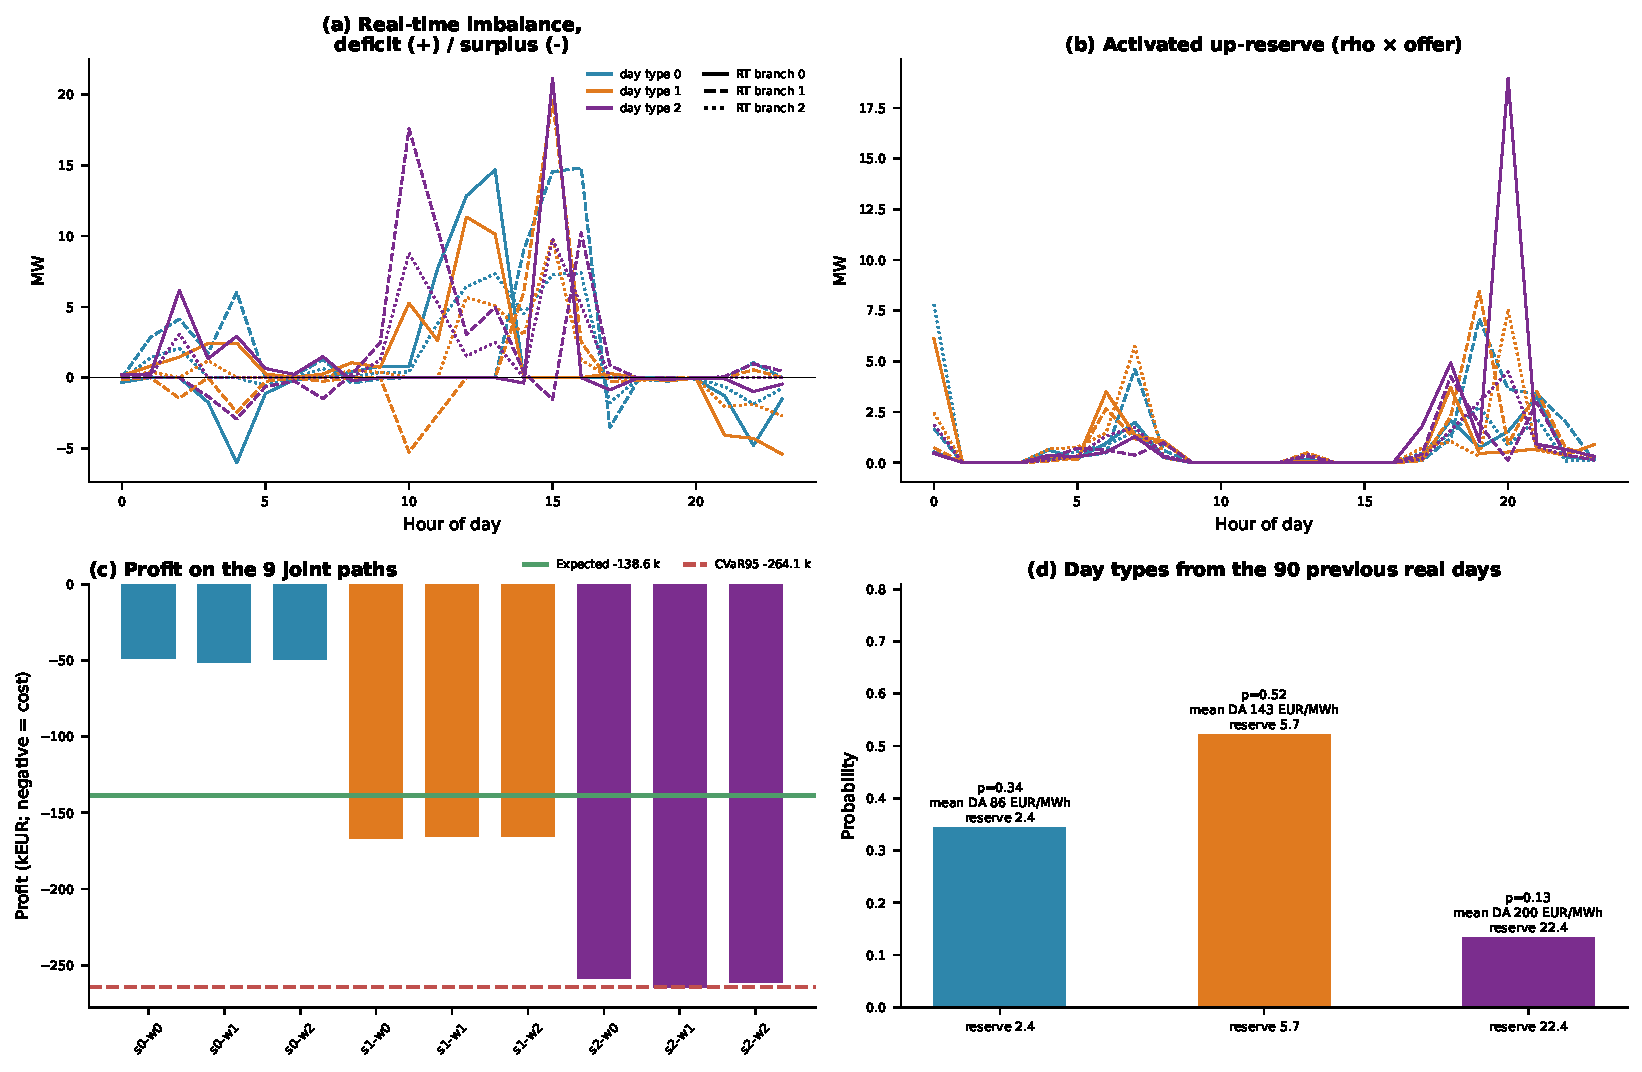
\includegraphics[width=0.82\textwidth]{Figures/fig_real_stage3.pdf}
\caption{Stage-3 outcomes on the nine joint paths $(s,w)$ of the reference tree: (a) real-time imbalance; (b) activated up-reserve; (c) profit of each path with the expected value and the CVaR$_{95}$; (d) probabilities and mean prices of the three day types built from the 90 preceding real days.}
\label{fig:stage3_recourse}
\end{figure*}

\subsection{Realized Performance on Actual Days}
The expected operating cost computed on the scenario tree (the in-tree expectation) is not the cost the plant would have met, so the Stage-1 decisions of each tree (production plan, gas turbine commitment, DA curves and reserve quantity) are fixed and evaluated on the actual prices of the following day, with Stage 2 and Stage 3 re-optimized (gap 0.5\%). The same is done for the DA-only plan and for the energy-only plan (DA plus ID, no reserve), so that savings are paired. Table~\ref{tab:realized} and Fig.~\ref{fig:dashboard}(d) give the result.

\begin{table}[t]
\caption{Expected (tree) versus realized savings on seven actual days, Stage-1 plan fixed (\euro, \% of the corresponding realized cost). Tree: expected saving on the training tree of each test day, solved with ID, real-time and activation shocks drawn with seed $2024+k$ (see text).}
\label{tab:realized}
\centering
\scriptsize
\setlength{\tabcolsep}{2.5pt}
\resizebox{\ifdim\width>\columnwidth\columnwidth\else\width\fi}{!}{%
\begin{tabular}{@{}lrrrr@{}}
\toprule
 & \multicolumn{2}{c}{\textbf{vs.\ Day-Ahead only}} & \multicolumn{2}{c}{\textbf{vs.\ no reserve (DA+ID)}} \\
\cmidrule(lr){2-3}\cmidrule(lr){4-5}
\textbf{Test day} & \textbf{Tree} & \textbf{Realized (\%)} & \textbf{Tree} & \textbf{Realized (\%)} \\
\midrule
2026-04-01 & 13,336 & 9,552 (4.1) & 10,868 & 7,869 (3.4) \\
2026-04-29 & 14,250 & 935 (2.1) & 12,043 & 199 (0.4) \\
2026-05-27 & 14,648 & 2,152 (7.0) & 11,946 & 512 (1.8) \\
2026-06-24 & 8,321 & 15,362 (9.6) & 6,765 & 4,428 (3.0) \\
2026-07-22 & 6,029 & $-$370 (-0.6) & 4,071 & 1,077 (1.8) \\
2026-08-19 & 4,257 & 7,053 (2.5) & 2,143 & 14,299 (4.9) \\
2026-09-16 & 5,240 & 3,136 (1.2) & 3,052 & 2,525 (1.0) \\
\midrule
\textbf{Mean} & 9,440 & 5,403 (3.7) & 7,270 & 4,415 (2.3) \\
\bottomrule
\end{tabular}}
\end{table}

The realized saving against DA only averages \euro 5,403 (3.7\%; median 2.5\%), against \euro 9,440 expected on the trees, and one day (22 July) is slightly negative. The reserve increment, i.e.\ the full plan against the DA+ID plan, is worth \euro 4,415 (2.3\%) against \euro 7,270 expected, positive on all seven days. Realized savings are below the expectation on five days and above it on two (24 June and 19 August), both high-price days (mean \euro 212 and 166/MWh).

The \emph{Tree} columns of Table~\ref{tab:realized} are not copies of Table~\ref{tab:market_ladder}. In the realized-performance test the training tree of the $k$-th test day ($k=0,\dots,6$) is solved with the ID, real-time and activation shocks drawn with seed $2024+k$, whereas the ladder of Table~\ref{tab:market_ladder} uses seed 2024 for every tree; the day types, their probabilities and the spinning reserve prices are identical. Only the first test day ($k=0$) therefore coincides with Table~\ref{tab:market_ladder} (\euro 13,336 in both). On the other six trees the expected saving differs by \euro 0.2--1.6k (for example \euro 14,648 against \euro 13,072 on 27 May, 12\%), and the mean over the seven trees is \euro 9,440 in Table~\ref{tab:realized} against \euro 9,186 in Table~\ref{tab:market_ladder}. The differences come from the ID and activation shocks and, to a smaller degree, from the 0.5\% MIP gap.

On 19 August the saving of the reserve plan against the DA+ID plan (\euro 14,299) is larger than its saving against the DA-only plan (\euro 7,053). This is not an arithmetic error. The three Stage-1 plans (DA only, DA+ID, DA+ID+reserve) are optimized separately and evaluated out of sample on the same day, so, unlike the in-tree savings, which can only increase as markets are added, the realized savings can decrease. On that day the realized cost was \euro 278,432 for the full plan, \euro 285,485 for the DA-only plan and \euro 292,731 for the DA+ID plan, so the DA+ID plan was \euro 7,246 worse than the DA-only plan, against a solver noise of about \euro 0.2k. The DA+ID plan was worse than the DA-only plan on two of the seven days (22 July and 19 August) and better on the other five (by \euro 0.6--10.9k).


Larger trees did not help. The mean realized cost of the plans from the $3\times3$, $6\times3$ and $12\times3$ trees is \euro 146,666, 148,028 and 147,748; the larger trees are worse by \euro 1,362 and \euro 1,082 on average and better on only one and two of the seven days, differences of the order of the evaluation tolerance (about \euro 0.7k). Comparing the expected operating cost on the tree (in-tree cost) with the cost of a single actual day is not a measure of tree quality, because day-to-day price level dominates it, so only paired differences are reported.


\subsection{Value of the Battery}
\label{sec:attribution}
\label{sec:battery}
This subsection separates the value of the battery by size and market, by reserve source, and by efficiency and degradation cost. All figures refer to the reference tree and to one day; they are not annualized and do not include investment cost.

\textit{Battery size.} Table~\ref{tab:battery_value} derives the value of the battery, Eq.~\eqref{eq:battery_value}, from the size sweep of Table~\ref{tab:coupling_sweep} (HiGHS, gap 0.5\%, noise \euro 294--401). The 40~MW/200~MWh battery lowers the expected operating cost by \euro 10,464 per day (7.0\% of the cost without a battery). The value grows less than proportionally with size, from \euro 63.7 to \euro 52.3 per installed MWh and day. Between 75\% and 83\% of it comes from DA and ID arbitrage and 17--25\% from reserve; the reserve share falls with size because the reserve value is limited by the spinning reserve price, which averages only \euro 6.79/MW/h on this tree. On trees with larger DA spreads (Table~\ref{tab:seasonal}) the arbitrage part is expected to differ; this was not run for the size sweep.

\begin{table}[t]
\caption{Value of the battery by size on the reference tree (\euro{} per day), derived from Table~\ref{tab:coupling_sweep}. $V_B$: total value (Eq.~\eqref{eq:battery_value}); $V_B^{\text{en}}$: DA+ID arbitrage part; $V_B^{\text{res}}$: reserve part; cost without battery: \euro 149,055 (DA+ID) and \euro 149,037 (all markets).}
\label{tab:battery_value}
\centering
\scriptsize
\setlength{\tabcolsep}{3pt}
\resizebox{\ifdim\width>\columnwidth\columnwidth\else\width\fi}{!}{%
\begin{tabular}{@{}lrrrrrrr@{}}
\toprule
\textbf{BESS (MW/MWh)} & \textbf{Cost DA+ID} & \textbf{Cost all} & $\boldsymbol{V_B}$ & $\boldsymbol{V_B^{\text{en}}}$ & $\boldsymbol{V_B^{\text{res}}}$ & \textbf{$V_B$ per MWh} & \textbf{$V_B$ (\%)} \\
\midrule
0/0     & 149,055 & 149,037 & 0      & 0     & 0     & --   & --  \\
10/50   & 146,658 & 145,850 & 3,187  & 2,397 & 790   & 63.7 & 2.1 \\
20/100  & 144,315 & 143,169 & 5,868  & 4,740 & 1,128 & 58.7 & 3.9 \\
40/200  & 140,396 & 138,573 & 10,464 & 8,659 & 1,805 & 52.3 & 7.0 \\
\bottomrule
\end{tabular}}
\end{table}

\textit{Reserve by asset.} Table~\ref{tab:reserve_assets} re-solves the reference tree with reserve allowed from different assets (HiGHS, gap 0.5\%, so differences below about \euro 0.7k are within the solver tolerance). The BESS alone captures \euro 1,639 of the \euro 1,823 reserve benefit (about 89\%); gas turbine and demand response alone recover \euro 261, which is below the resolution, as is the difference of \euro 184 between the BESS-only and the four-asset case.

\begin{table}[t]
\caption{expected net operating cost by reserve source (EUR, reference tree, Stage-1 reserve, real spinning reserve prices).}
\label{tab:reserve_assets}
\centering
\scriptsize
\resizebox{\ifdim\width>\columnwidth\columnwidth\else\width\fi}{!}{%
\begin{tabular}{@{}lrrr@{}}
\toprule
\textbf{Reserve allowed from} & \textbf{Net cost} & \textbf{Saving vs.\ none} & \textbf{Avg. offer (MW)} \\
\midrule
none (DA+ID only) & 140,396.30 & -- & 0.0 \\
GT + DR only & 140,135.00 & 261.30 & 0.7 \\
BESS only (dis + ch) & 138,757.03 & 1,639.27 & 8.5 \\
all four & 138,573.01 & 1,823.29 & 10.3 \\
\bottomrule
\end{tabular}}
\end{table}

\textit{Efficiency and degradation cost.} Table~\ref{tab:battery_sens} re-solves the three market levels on the reference tree for round-trip efficiencies of 76\% (base case, $\eta_{\text{ch}}=0.80$, $\eta_{\text{dis}}=0.95$), 85\% and 90\% (symmetric $\eta_{\text{ch}}=\eta_{\text{dis}}$) and for degradation costs $C_{\text{TP}}$ of 2.5, 5 and 10~\euro/MWh (Gurobi, gap 0.2\%). Three results follow.
\begin{enumerate}
    \item The reserve saving is stable. It lies between \euro 1,863 and \euro 2,054 in all nine cells, a spread of \euro 191 that is within the solver tolerance of \euro 492--572, so the reserve saving is effectively constant.
    \item The total saving against DA only varies between 2.86\% and 3.14\% (\euro 3,940--4,546). It rises slightly with $C_{\text{TP}}$ and falls slightly with efficiency, because the DA-only reference benefits more from a better battery than the full plan does: from 76\% to 90\% efficiency at \euro 5/MWh the Level-1 cost falls by \euro 3,881 and the Level-3 cost by \euro 3,593. Differences of \euro 0.1--0.6k are of the order of the noise and are not interpreted individually.
    \item The cost level depends strongly on the battery parameters. Raising the efficiency from 76\% to 90\% at \euro 5/MWh lowers the Level-3 cost by \euro 3,593 (2.6\%), nearly twice the reserve saving, and raising $C_{\text{TP}}$ from \euro 2.5 to \euro 10/MWh at 76\% raises it by \euro 2,863 (2.1\%).
\end{enumerate}
The battery supplies 86--91\% of the offered reserve capacity in every cell. This is a share of the offered MW, not of the value; the value attribution of Table~\ref{tab:reserve_assets} was computed at the base case only. The reserve value of the battery is therefore a robust feature of this tree, while the cost level is a first-order function of the battery efficiency.

\begin{table*}[t]
\caption{Sensitivity of the market ladder to the battery round-trip efficiency (RTE, \%) and degradation cost $C_{\text{TP}}$ (\euro/MWh), reference tree (\euro{} per day). Gurobi, gap $\le 0.2\%$. Offer: mean reserve offer (MW); BESS: share of the offer supplied by the battery (\%); Noise = (sum of the gaps of Levels 1 and 3) $\times$ Level-1 cost. The base case is RTE 76\%, $C_{\text{TP}}=5$.}
\label{tab:battery_sens}
\centering
\scriptsize
\setlength{\tabcolsep}{4pt}
\begin{tabular}{@{}rrrrrrrrrrr@{}}
\toprule
\textbf{RTE} & $\boldsymbol{C_{\text{TP}}}$ & \textbf{L1} & \textbf{L2} & \textbf{L3} & \textbf{ID saving} & \textbf{Res.\ saving} & \textbf{Total (\%)} & \textbf{Offer} & \textbf{BESS} & \textbf{Noise} \\
\midrule
76 & 2.5 & 141,509 & 139,293 & 137,306 & 2,216 & 1,987 & 4,203 (2.97) & 9.1 & 89 & 565 \\
76 & 5 & 142,700 & 140,277 & 138,414 & 2,423 & 1,863 & 4,286 (3.00) & 10.2 & 89 & 492 \\
76 & 10 & 144,715 & 142,138 & 140,169 & 2,576 & 1,969 & 4,546 (3.14) & 11.0 & 89 & 572 \\
85 & 2.5 & 139,005 & 136,943 & 134,955 & 2,062 & 1,988 & 4,051 (2.91) & 9.0 & 90 & 535 \\
85 & 5 & 140,229 & 138,164 & 136,110 & 2,065 & 2,054 & 4,119 (2.94) & 9.0 & 90 & 559 \\
85 & 10 & 142,668 & 140,419 & 138,405 & 2,250 & 2,014 & 4,263 (2.99) & 9.2 & 91 & 566 \\
90 & 2.5 & 137,583 & 135,512 & 133,643 & 2,071 & 1,869 & 3,940 (2.86) & 9.0 & 86 & 549 \\
90 & 5 & 138,819 & 136,753 & 134,821 & 2,066 & 1,932 & 3,998 (2.88) & 9.0 & 87 & 553 \\
90 & 10 & 141,283 & 139,154 & 137,118 & 2,130 & 2,036 & 4,166 (2.95) & 9.0 & 90 & 559 \\
\bottomrule
\end{tabular}
\end{table*}


\subsection{Value of the Stochastic Solution}
\label{sec:vss}
The stochastic formulation is justified only if it beats the plan that a planner would obtain from a model with mean prices. For each of the eleven trees (the eight trees of Table~\ref{tab:market_ladder} and the three winter trees of Table~\ref{tab:winter_ladder}) the SP value, the EV problem and the EEV value of Eqs.~\eqref{eq:rp}--\eqref{eq:vss} were solved at Level 3 with Gurobi and a gap of 0.5\%. The Stage-1 decisions of the EV problem, i.e.\ the EV plan (batch starts, gas-turbine commitment, DA quantities and hourly reserve quantity), are fixed in the full $3\times3$ tree, and Stage 2 and Stage 3 are re-optimized, which gives the EEV. The SP values equal the Level-3 costs of Table~\ref{tab:market_ladder} on seven trees; on the reference tree the Gurobi value is \euro 138,414 against \euro 138,573 from HiGHS (0.1\%, inside the gap).

\begin{table*}[t]
\caption{Value of the stochastic solution at Level 3 (\euro{} per day; \% of SP in brackets). SP: optimal expected operating cost of the stochastic problem; EEV: expected operating cost of the EV plan fixed in the full tree (Eq.~\eqref{eq:eev}); VSS = EEV $-$ SP; Noise: (sum of the two gaps) $\times$ SP; $^{\ast}$: VSS within the solver tolerance. Offer: mean reserve offer of the stochastic (SP) plan / EV plan (MW). Gurobi, gap 0.5\%. The first block is the eight trees of Table~\ref{tab:market_ladder}, the second the three winter trees of Table~\ref{tab:winter_ladder}.}
\label{tab:vss}
\centering
\scriptsize
\setlength{\tabcolsep}{4pt}
\begin{tabular}{@{}lrrrrr@{}}
\toprule
\textbf{History end} & \textbf{SP} & \textbf{EEV} & \textbf{VSS (\%)} & \textbf{Noise} & \textbf{Offer SP / EV} \\
\midrule
2026-03-31 & 158,601 & 159,849 & 1,247 (0.79) & 337 & 36.9 / 43.5 \\
2026-04-28 & 126,779 & 128,155 & 1,377 (1.09) & 647 & 37.3 / 41.3 \\
2026-05-26 & 96,816 & 97,747 & 931 (0.96) & 483 & 34.9 / 33.9 \\
2026-06-23 & 86,923 & 87,753 & 830$^{\ast}$ (0.95) & 866 & 22.4 / 21.5 \\
2026-07-21 & 89,278 & 90,154 & 876 (0.98) & 402 & 23.6 / 21.1 \\
2026-08-18 & 90,707 & 91,427 & 720 (0.79) & 454 & 12.7 / 16.5 \\
2026-09-15 & 114,706 & 116,156 & 1,450 (1.26) & 573 & 11.4 / 15.4 \\
2026-10-11 & 138,414 & 139,397 & 983 (0.71) & 705 & 10.2 / 10.7 \\
\midrule
Mean (8 trees) & & & 1,052 (0.94) & 558 & \\
\midrule
2025-12-31 & 133,574 & 134,545 & 971 (0.73) & 667 & 32.3 / 33.9 \\
2026-01-28 & 146,598 & 148,284 & 1,686 (1.15) & 732 & 32.8 / 34.0 \\
2026-02-25 & 155,871 & 156,915 & 1,043 (0.67) & 775 & 32.3 / 32.2 \\
\midrule
Mean (3 winter trees) & & & 1,233 (0.85) & 725 & \\
Mean (11 trees) & & & 1,101 (0.92) & 604 & \\
\bottomrule
\end{tabular}
\end{table*}

The VSS is positive on all eleven trees, between \euro 720 and \euro 1,686 (0.67--1.26\% of SP), with a mean of \euro 1,052 (0.94\%) on the eight trees, \euro 1,233 (0.85\%) on the three winter trees and \euro 1,101 (0.92\%) over all eleven. It exceeds the solver noise on 10 of 11 trees; the exception is 23 June (\euro 830 against \euro 866). On the eight trees the EV plan retains \euro 7,521 of the \euro 8,573 multi-market saving against DA only (88\%, with all eight trees solved with Gurobi); the share is 90--93\% on the four earliest trees, 84--86\% in July and August, and 69\% and 77\% on 15 September and 11 October, the trees with the lowest spinning reserve prices.


\subsection{Production Coupling}
\label{sec:coupling}
The integrated model is compared with a decoupled benchmark in which the production plan is first fixed from the energy-only Day-Ahead + Intraday optimum (plan A) or from the DA-only optimum (plan B), and the offer curves, ID, BESS, gas turbine and reserve decisions are then re-optimized with that plan held fixed. The coupling value is the decoupled minus the integrated cost; since the decoupled problem is a restriction, values within the solver tolerance are treated as zero. Table~\ref{tab:coupling_sweep} repeats the comparison for several battery sizes on the reference tree: the reserve benefit grows with battery size, from \euro 18 without a battery to \euro 1,823 at 40~MW/200~MWh, but the coupling value is within the solver tolerance at every size ($-$111 to +208 against a noise of 294--401) and shows no trend. Plan B gives +112 at 40/200~MWh.

\begin{table}[t]
\caption{Reserve benefit and production-coupling value versus battery size (EUR, reference tree, Stage-1 reserve, plan A).}
\label{tab:coupling_sweep}
\centering
\scriptsize
\setlength{\tabcolsep}{2.5pt}
\resizebox{\ifdim\width>\columnwidth\columnwidth\else\width\fi}{!}{%
\begin{tabular}{@{}lrrrrrrr@{}}
\toprule
\textbf{BESS (MW/MWh)} & \textbf{No reserve} & \textbf{Integrated} & \textbf{Decoupled} & \textbf{Coupling} & \textbf{Res. benefit} & \textbf{Noise} & \textbf{Offer (MW)} \\
\midrule
0/0 & 149,055 & 149,037 & 149,037 & 0.0 & 18 & 294 & 0.2 \\
10/50 & 146,658 & 145,850 & 146,057 & 207.6 & 808 & 330 & 3.0 \\
20/100 & 144,315 & 143,169 & 143,201 & 32.5 & 1,147 & 401 & 5.6 \\
40/200 & 140,396 & 138,573 & 138,462 & $-$110.5 & 1,823 & 313 & 10.3 \\
\bottomrule
\end{tabular}}
\end{table}

The reference tree alone could suggest that coupling is always negligible, so the decoupling test was repeated on earlier trees (Table~\ref{tab:coupling_dates}). These runs use real spinning reserve prices from DK1 but the reserve as a price-quantity curve; the Stage-1 version was run on the reference tree only. The coupling value is \euro 682, 1,333 and 718 on three of the four earlier trees (0.4--1.4\% of cost), above the noise on each, and $-$94 (noise 281) on the fourth. Planning production separately from the market offers therefore raises the cost by 0.4--1.4\% on three of the four earlier trees; on the fourth tree the difference is within the solver tolerance, and no negative value exceeds it. On the reference tree, with the Stage-1 reserve used in the rest of the paper, the difference is $-$0.1\% and also within the solver tolerance.

\begin{table}[t]
\caption{Production-coupling value on several real trees (EUR; \% of integrated cost; plan A unless stated). ``Curve'' = reserve as price-quantity curve, ``Stage-1'' = single quantity.}
\label{tab:coupling_dates}
\centering
\scriptsize
\setlength{\tabcolsep}{2.5pt}
\resizebox{\ifdim\width>\columnwidth\columnwidth\else\width\fi}{!}{%
\begin{tabular}{@{}llrrrrr@{}}
\toprule
\textbf{History end} & \textbf{Reserve} & \textbf{Integrated} & \textbf{Decoupled A} & \textbf{Coupling A (\%)} & \textbf{Noise} & \textbf{Coupling B} \\
\midrule
2026-03-31 & Curve & 156,876 & 157,557 & 682 (0.4) & 90 & 942 \\
2026-04-28 & Curve & 125,691 & 125,597 & $-$94 (-0.1) & 281 & 256 \\
2026-05-26 & Curve & 95,765 & 97,097 & 1,332 (1.4) & 331 & 1,160 \\
2026-06-23 & Curve & 86,683 & 87,400 & 718 (0.8) & 172 & 1,527 \\
2026-10-11 & Stage-1 & 138,573 & 138,462 & $-$111 (-0.1) & 313 & 112 \\
\bottomrule
\end{tabular}}
\end{table}

\subsection{Robustness: Reserve Price and Risk}
\label{sec:robustness}
\textit{Reserve-price source and sensitivity.} Real spinning reserve capacity prices on the reference tree average only 5.2\% of the DA price (\euro 6.79/MWh against \euro 15.7/MWh), and they are concentrated on a few days. Table~\ref{tab:reserve_price} shows the effect on the reference tree (DA only: \euro 142,700.24): with the real spinning reserve prices the saving is 3.60\% when the reserve is a price-quantity curve, and 2.89\% when it is committed as a single Stage-1 quantity. Scaling the real series by 0.5 and 1.5 gives 2.03\% and 4.15\%, so the saving is not proportional to the price (a factor of 2.0 between the extremes) because the plant also offers more reserve (5.1 to 12.1~MW). The price-quantity curve (first row) is an upper bound for what a price-quantity bid could earn and the Stage-1 quantity a conservative bound.

\begin{table}[t]
\caption{Reserve-price source and sensitivity, reference tree. Savings are against DA only (\euro 142,700.24).}
\label{tab:reserve_price}
\centering
\scriptsize
\setlength{\tabcolsep}{2.5pt}
\resizebox{\ifdim\width>\columnwidth\columnwidth\else\width\fi}{!}{%
\begin{tabular}{@{}lrrr@{}}
\toprule
\textbf{Reserve price / commitment} & \textbf{Net cost (\euro)} & \textbf{Saving (\euro, \%)} & \textbf{Offer (MW)} \\
\midrule
Real spinning reserve, price-quantity curve & 137,568.68 & 5,131.55 (3.60) & 9.9 \\
Real spinning reserve, Stage-1 quantity ($\times1.0$) & 138,573.01 & 4,127.23 (2.89) & 10.3 \\
Real spinning reserve, Stage-1 quantity ($\times0.5$) & 139,800.01 & 2,900.23 (2.03) & 5.1 \\
Real spinning reserve, Stage-1 quantity ($\times1.5$) & 136,774.52 & 5,925.72 (4.15) & 12.1 \\
\bottomrule
\end{tabular}}
\end{table}

\textit{Risk aversion.} To show that the formulation supports
risk aversion, Table~\ref{tab:frontier} gives the CVaR$_{95}$ frontier on a $12\times2$ tree built from the same history (24 paths, gap at most 1\%). With 24 paths the 5\% tail is 1.2 paths wide, so CVaR equals the worst path. Moving from $\beta=0$ to $\beta=0.9$ raises the expected operating cost by \euro 6,877 (4.9\%), improves CVaR$_{95}$ by \euro 13,298 (4.8\%) and lowers the standard deviation by 11\%. CVaR improves with every step of $\beta$, but the step from $\beta=0.5$ to $0.75$ is only \euro 368, within solver tolerance, so the frontier is indicative; the average reserve offer is not monotone in $\beta$ (5.8--15.4~MW, lowest at $\beta=0.25$).

\begin{table}[t]
\caption{CVaR frontier on a $12\times2$ tree, reference history ($\alpha=0.95$; net operating cost in \euro{} per day, lower is better).}
\label{tab:frontier}
\centering
\scriptsize
\resizebox{\ifdim\width>\columnwidth\columnwidth\else\width\fi}{!}{%
\begin{tabular}{@{}rrrrr@{}}
\toprule
$\beta$ & \textbf{Exp. cost} & \textbf{CVaR$_{95}$ of cost} & \textbf{Std.} & \textbf{Avg. reserve (MW)} \\
\midrule
0    & 138,996.35 & 276,681.57 & 84,699.11 & 6.5 \\
0.25 & 139,681.30 & 272,188.78 & 83,357.63 & 5.8 \\
0.5  & 143,280.32 & 265,437.38 & 77,922.49 & 12.3 \\
0.75 & 145,629.56 & 265,069.36 & 75,943.04 & 12.6 \\
0.9  & 145,872.92 & 263,383.52 & 75,375.00 & 15.4 \\
\bottomrule
\end{tabular}}
\end{table}

\subsection{Production Rescheduling after DA Clearing}\label{sec:resched}
Once the DA prices of the test day are published, the curves are applied as step functions and the DA quantities are booked. Stage 2 and Stage 3 are then re-optimized on the actual day with the jobs either kept as in Stage 1 (baseline) or allowed to move by at most $\pm3$ h on the same machine (``strict'' rescheduling), so any mismatch between the booked energy and the new load is paid in the ID and imbalance settlement. Table~\ref{tab:rescheduling_results} and Fig.~\ref{fig:dashboard}(c) show the result for the seven test days.

\begin{table}[t]
\caption{Production rescheduling after Day-Ahead clearing (strict: same machine and task, start shifted by at most $\pm3$ h; \euro, daily saving in \% of the daily baseline cost; the mean row gives the mean saving in \% of the mean baseline). Noise = (sum of the two MIP gaps) $\times$ baseline cost.}
\label{tab:rescheduling_results}
\centering
\scriptsize
\setlength{\tabcolsep}{2.5pt}
\resizebox{\ifdim\width>\columnwidth\columnwidth\else\width\fi}{!}{%
\begin{tabular}{@{}lrrrrr@{}}
\toprule
\textbf{Test day} & \textbf{Baseline} & \textbf{Rescheduled} & \textbf{Saving (\%)} & \textbf{Jobs moved} & \textbf{Noise} \\
\midrule
2026-04-01 & 225,690 & 219,967 & 5,723 (2.5) & 7 & 1,510 \\
2026-04-29 & 45,880 & 40,998 & 4,881 (10.6) & 13 & 281 \\
2026-05-27 & 28,785 & 27,042 & 1,743 (6.1) & 12 & 37 \\
2026-06-24 & 144,835 & 143,014 & 1,821 (1.3) & 9 & 1,257 \\
2026-07-22 & 57,899 & 56,195 & 1,704 (2.9) & 13 & 288 \\
2026-08-19 & 280,025 & 277,925 & 2,099 (0.7) & 7 & 1,615 \\
2026-09-16 & 252,868 & 250,673 & 2,194 (0.9) & 2 & 1,722 \\
\midrule
\textbf{Mean} & 147,997 & 145,116 & \textbf{2,881} (1.9) & 9.0 & 959 \\
\bottomrule
\end{tabular}}
\end{table}

The saving averages \euro 2,881 per day, about 1.9\% of the mean baseline cost of \euro 147,997, and is above the estimated noise on all seven days, by less than \euro 0.6k on three of them. The daily percentages are inflated on low-cost days (29~April, 27~May), so the euro value and the percentage of the mean baseline are the more reliable measures. ID prices in this test are modelled as in Section~\ref{sec:casestudy}, and the saving is measured against a fixed job plan; it is not fed back into the offering objective and must not be added to the ladder saving.


\section{Discussion}
\label{sec:discussion}
\textit{Where the battery value comes from.} On the reference tree, 83\% of the battery value is DA and ID arbitrage and 17\% is reserve. The reserve part is small on this tree because the spinning reserve price is low (\euro 6.79 MWh), but it is the part that depends most on the market: the reserve saving of the ladder falls from \euro 12.1k to \euro 1.8k as the 90-day mean spinning reserve price falls from about \euro 20 to \euro 7 MWh. A battery business case based on the reserve market is therefore exposed to the reserve price, while the arbitrage part depends on the DA spread, which is large in spring and summer and small in winter (Table~\ref{tab:seasonal}).

\textit{Efficiency matters for the cost level more than for the market saving.} The sensitivity grid shows that the reserve saving and the multi-market saving hardly change with efficiency and degradation cost, whereas the cost level changes by \euro 3.6k per day between 76\% and 90\% round-trip efficiency. For a plant owner, the efficiency of the battery is thus a larger economic lever than the choice of whether to add the reserve market.

\textit{Contribution of the stochastic formulation and of joint production planning.} The VSS is 0.7--1.3\% of the expected operating cost (mean 0.9\%). Although modest in magnitude, it exceeds the solver tolerance on 10 of the 11 trees, so the stochastic Stage-1 plan outperforms the plan derived from mean prices in nearly all cases. Planning production jointly with the market offers, instead of fixing the production schedule beforehand, reduces the expected cost by 0.4--1.4\% on three of the four earlier trees. On the fourth tree and on the reference tree, the difference lies within the solver tolerance and cannot be distinguished from zero. These effects are small in comparison with the savings obtained from multi-market participation (2.9--11.9\%) and with the value of the battery (7.0\% of the expected cost on the reference tree). For the plant considered here, the market participation and the battery operation therefore determine most of the economic result, whereas the discrete production schedule contributes a smaller, second-order effect that depends on the date.


\section{Conclusion}
\label{sec:conclusion}
A three-stage stochastic MILP for a batch-production prosumer with a gas turbine and a battery was evaluated on one year of real DK1 DA prices and real spinning reserve capacity prices, with the reserve committed as a Stage-1 quantity. Four findings answer the questions of the Introduction.
\begin{enumerate}
    \item \textbf{Q1.} On eight scenario trees, Intraday trading and up-reserve reduce the expected net operating cost by 2.9--11.9\% (mean 7.1\%) against DA only; the reserve part follows the spinning reserve capacity price, which fell during the year.
    \item \textbf{Q2.} On seven actual days the realized saving is 3.7\% (\euro 5,403) on average.
    \item \textbf{Q3.} On the reference tree the 40~MW/200~MWh battery lowers the expected operating cost by \euro 10.5k per day (7.0\%), 83\% from DA and ID arbitrage and 17\% from reserve, and the battery supplies about 89\% of the offered reserve capacity (9.2 of 10.3~MW). The reserve saving stays at \euro 1.9--2.1k for round-trip efficiencies of 76--90\% and degradation costs of \euro 2.5--10/MWh, while the cost level changes by \euro 3.6k per day with the efficiency.
    \item \textbf{Q4.} The SP plan beats the deterministic expected-value (EV) plan by 0.7--1.3\% (mean 0.9\%), i.e.\ the VSS = EEV $-$ SP, above the solver noise on 10 of 11 trees. Planning production separately from the market offers raises the cost by 0.4--1.4\% on three of four earlier trees and is within the solver tolerance on the fourth tree and on the reference tree. Rescheduling jobs by $\pm3$~h after Day-Ahead clearing is worth \euro 2,881 per day (about 1.9\% of the mean baseline cost) in a separate test that is not additive to the ladder.
\end{enumerate}
\textbf{Future work.} The values are per day for one representative plant and do not include investment cost, so they support a comparison of strategies and battery parameters rather than an investment appraisal.Future work will use real Intraday and imbalance settlement and reserve-activation prices, calibrate the
gas-turbine fuel cost to gas and carbon prices, handle negative DA  prices
explicitly, carry out a calibrated risk analysis with a finer scenario tree and
$\alpha=0.8$--$0.9$, and extend the evaluation to a longer rolling horizon with
annualized values and non-linear battery ageing models. 


\section*{CRediT authorship contribution statement}
\textbf{Sreelatha Aihloor Subramanyam:} Conceptualization, Methodology, Software, Validation, Formal analysis, Investigation, Data curation, Visualization, Writing -- original draft. \textbf{Amjad Anvari-Moghaddam:} Conceptualization, Supervision, Project administration, Resources, Writing -- review \& editing.

\section*{Declaration of competing interest}
% TODO: confirm.
The authors declare that they have no known competing financial interests or personal relationships that could have appeared to influence the work reported in this paper. 

\section*{Funding}
This work was supported by European Regional Development Fund: under grant [grant number].

\section*{Data availability}
The DK1 Day-Ahead and spinning reserve capacity prices are public (Nord Pool via Energi Data Service). The source code, price extracts, result tables, run logs and the scripts for all tables and figures, including the VSS and battery-sensitivity runs (\texttt{tier2\_real.py}), are available at \url{https://github.com/sreelatha217-ux/Multistage_Flextrade/tree/main/Offering_Strategy_Handoff}.

\section*{Declaration of generative AI and AI-assisted technologies in the writing process}
During manuscript preparation the authors used Claude (Anthropic) for language editing, and take full responsibility for the content after reviewing and editing it.

\bibliographystyle{elsarticle-num}
\bibliography{references}


\end{document}
